
%%%%%%%%%%%%%%%%%%%%%%%%%%%%%%%%%%%%%%%%%%%%%%%%%%%%%%%%%%%%%%%%%%
\section{Synchronous machine drives -- basic models and control concepts}
%%%%%%%%%%%%%%%%%%%%%%%%%%%%%%%%%%%%%%%%%%%%%%%%%%%%%%%%%%%%%%%%%%

%%%%%%%%%%%%%%%%%%%%%%%%%%%%%%%%%%%%%%%%%%%%%%%%%%%%%%%%%%%%%%%%%%
\subsection{Synchronous machine models}
%%%%%%%%%%%%%%%%%%%%%%%%%%%%%%%%%%%%%%%%%%%%%%%%%%%%%%%%%%%%%%%%%%

%%%%%%%%%%%%%%%%%%%%%%%%%%%%%%%%%%%%%%%%%%%%%%%%%%%%%%%%%%%%%
%% Synchronous machine (SM) rotor types %%
%%%%%%%%%%%%%%%%%%%%%%%%%%%%%%%%%%%%%%%%%%%%%%%%%%%%%%%%%%%%%
\begin{frame}
    \frametitle{Permanent magnet synchronous machine (PMSM) rotor types}
    \begin{figure}
        \centering
        \begin{subfigure}{0.49\textwidth}
            \centering
            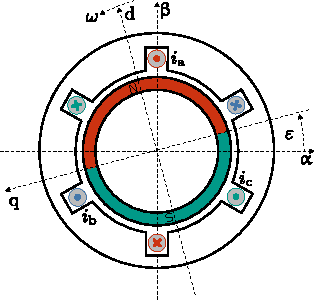
\includegraphics[width=0.8\textwidth]{fig/lec03/SPMSM.pdf}
            \caption{Surface-mounted PMSM(SPMSM)}
        \end{subfigure}
        \hfill
        \begin{subfigure}{0.49\textwidth}
            \centering
            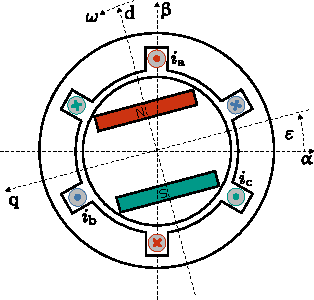
\includegraphics[width=0.8\textwidth]{fig/lec03/IPMSM.pdf}
            \caption{Interior PMSM (IPMSM)}
        \end{subfigure}
        \caption{Major rotor types of permanent magnet synchronous machines (PMSM) with dq reference frame axes aligned to the rotor flux produced by the permanent magnets}
        \label{fig:examples_PMSM_rotor}
    \end{figure}
\end{frame}

%%%%%%%%%%%%%%%%%%%%%%%%%%%%%%%%%%%%%%%%%%%%%%%%%%%%%%%%%%%%%
%% Summary: PMSM model in dq coordinates   %%
%%%%%%%%%%%%%%%%%%%%%%%%%%%%%%%%%%%%%%%%%%%%%%%%%%%%%%%%%%%%%
\begin{frame}
    \frametitle{PMSM model in dq coordinates}
    The most important equations of the PMSM model in the  dq coordinates are\footnote{A detailed derivation can be found in \href{https://github.com/IAS-Uni-Siegen/EMD_course}{Fundamentals of electrical machines and drives (EMD) course}.}:
    \begin{equation}
        \begin{alignedat}{4}
             &  & \mbox{Stator voltage:} &  & \quad\bm{u}_\mathrm{s,dq}( & t) &  & = R_\mathrm{s} \bm{i}_\mathrm{s,dq}(t)+ \omega(t)\bm{J}\bm{\psi}_\mathrm{s,dq}(t) + \nicefrac{\mathrm{d}}{\mathrm{d}t}\bm{\psi}_\mathrm{s,dq}(t), \\
            \onslide<2->{&  & \mbox{Stator flux linkage:} &  & \quad \bm{\psi}_\mathrm{s,dq}( & t) &  & = \bm{f}_{\psi_\mathrm{s}}(\bm{i}_\mathrm{s,dq}(t), \psi_\mathrm{PM}),}                                                      \\\onslide<3->{
                                                                                                                                                                                                                                                          &  & \mbox{Torque:}              &  & \quad T(                       & t) &  & = \nicefrac{3}{2} p (\bm{i}_\mathrm{s,dq}(t))\T\bm{J}\bm{\psi}_\mathrm{s,dq}(t)}
        \end{alignedat}
        \label{eq:basic_PMSM_model_set}
    \end{equation}
    \onslide<4->{with the further signals and parameters:
            \begin{equation*}
                \begin{aligned}
                    \bm{i}_\mathrm{s,dq}: \text{stator current},                                                              &
                    \qquad \psi_\mathrm{PM}  : \text{permanent magnet flux linkage},                                            \\
                    R_\mathrm{s}:                                                          \text{stator winding resistances}, &
                    \qquad \bm{f}_{\psi_\mathrm{s}} : \text{stator flux linkage function},                                      \\
                    p                                           : \text{pole pair number},                                    &
                    \qquad \omega = p\omega_\mathrm{me}                   : \text{electrical angular velocity,}                 \\
                    \bm{J}: \text{90° rotation matrix, cf. \eqref{eq:J_rotation}}.                                            &
                \end{aligned}
            \end{equation*}}
\end{frame}

%%%%%%%%%%%%%%%%%%%%%%%%%%%%%%%%%%%%%%%%%%%%%%%%%%%%%%%%%%%%%
%% Flux saturation motor cross section %%
%%%%%%%%%%%%%%%%%%%%%%%%%%%%%%%%%%%%%%%%%%%%%%%%%%%%%%%%%%%%%

\begin{frame}
    \frametitle{Flux saturation in electric machines}
    \begin{figure}
        \centering
        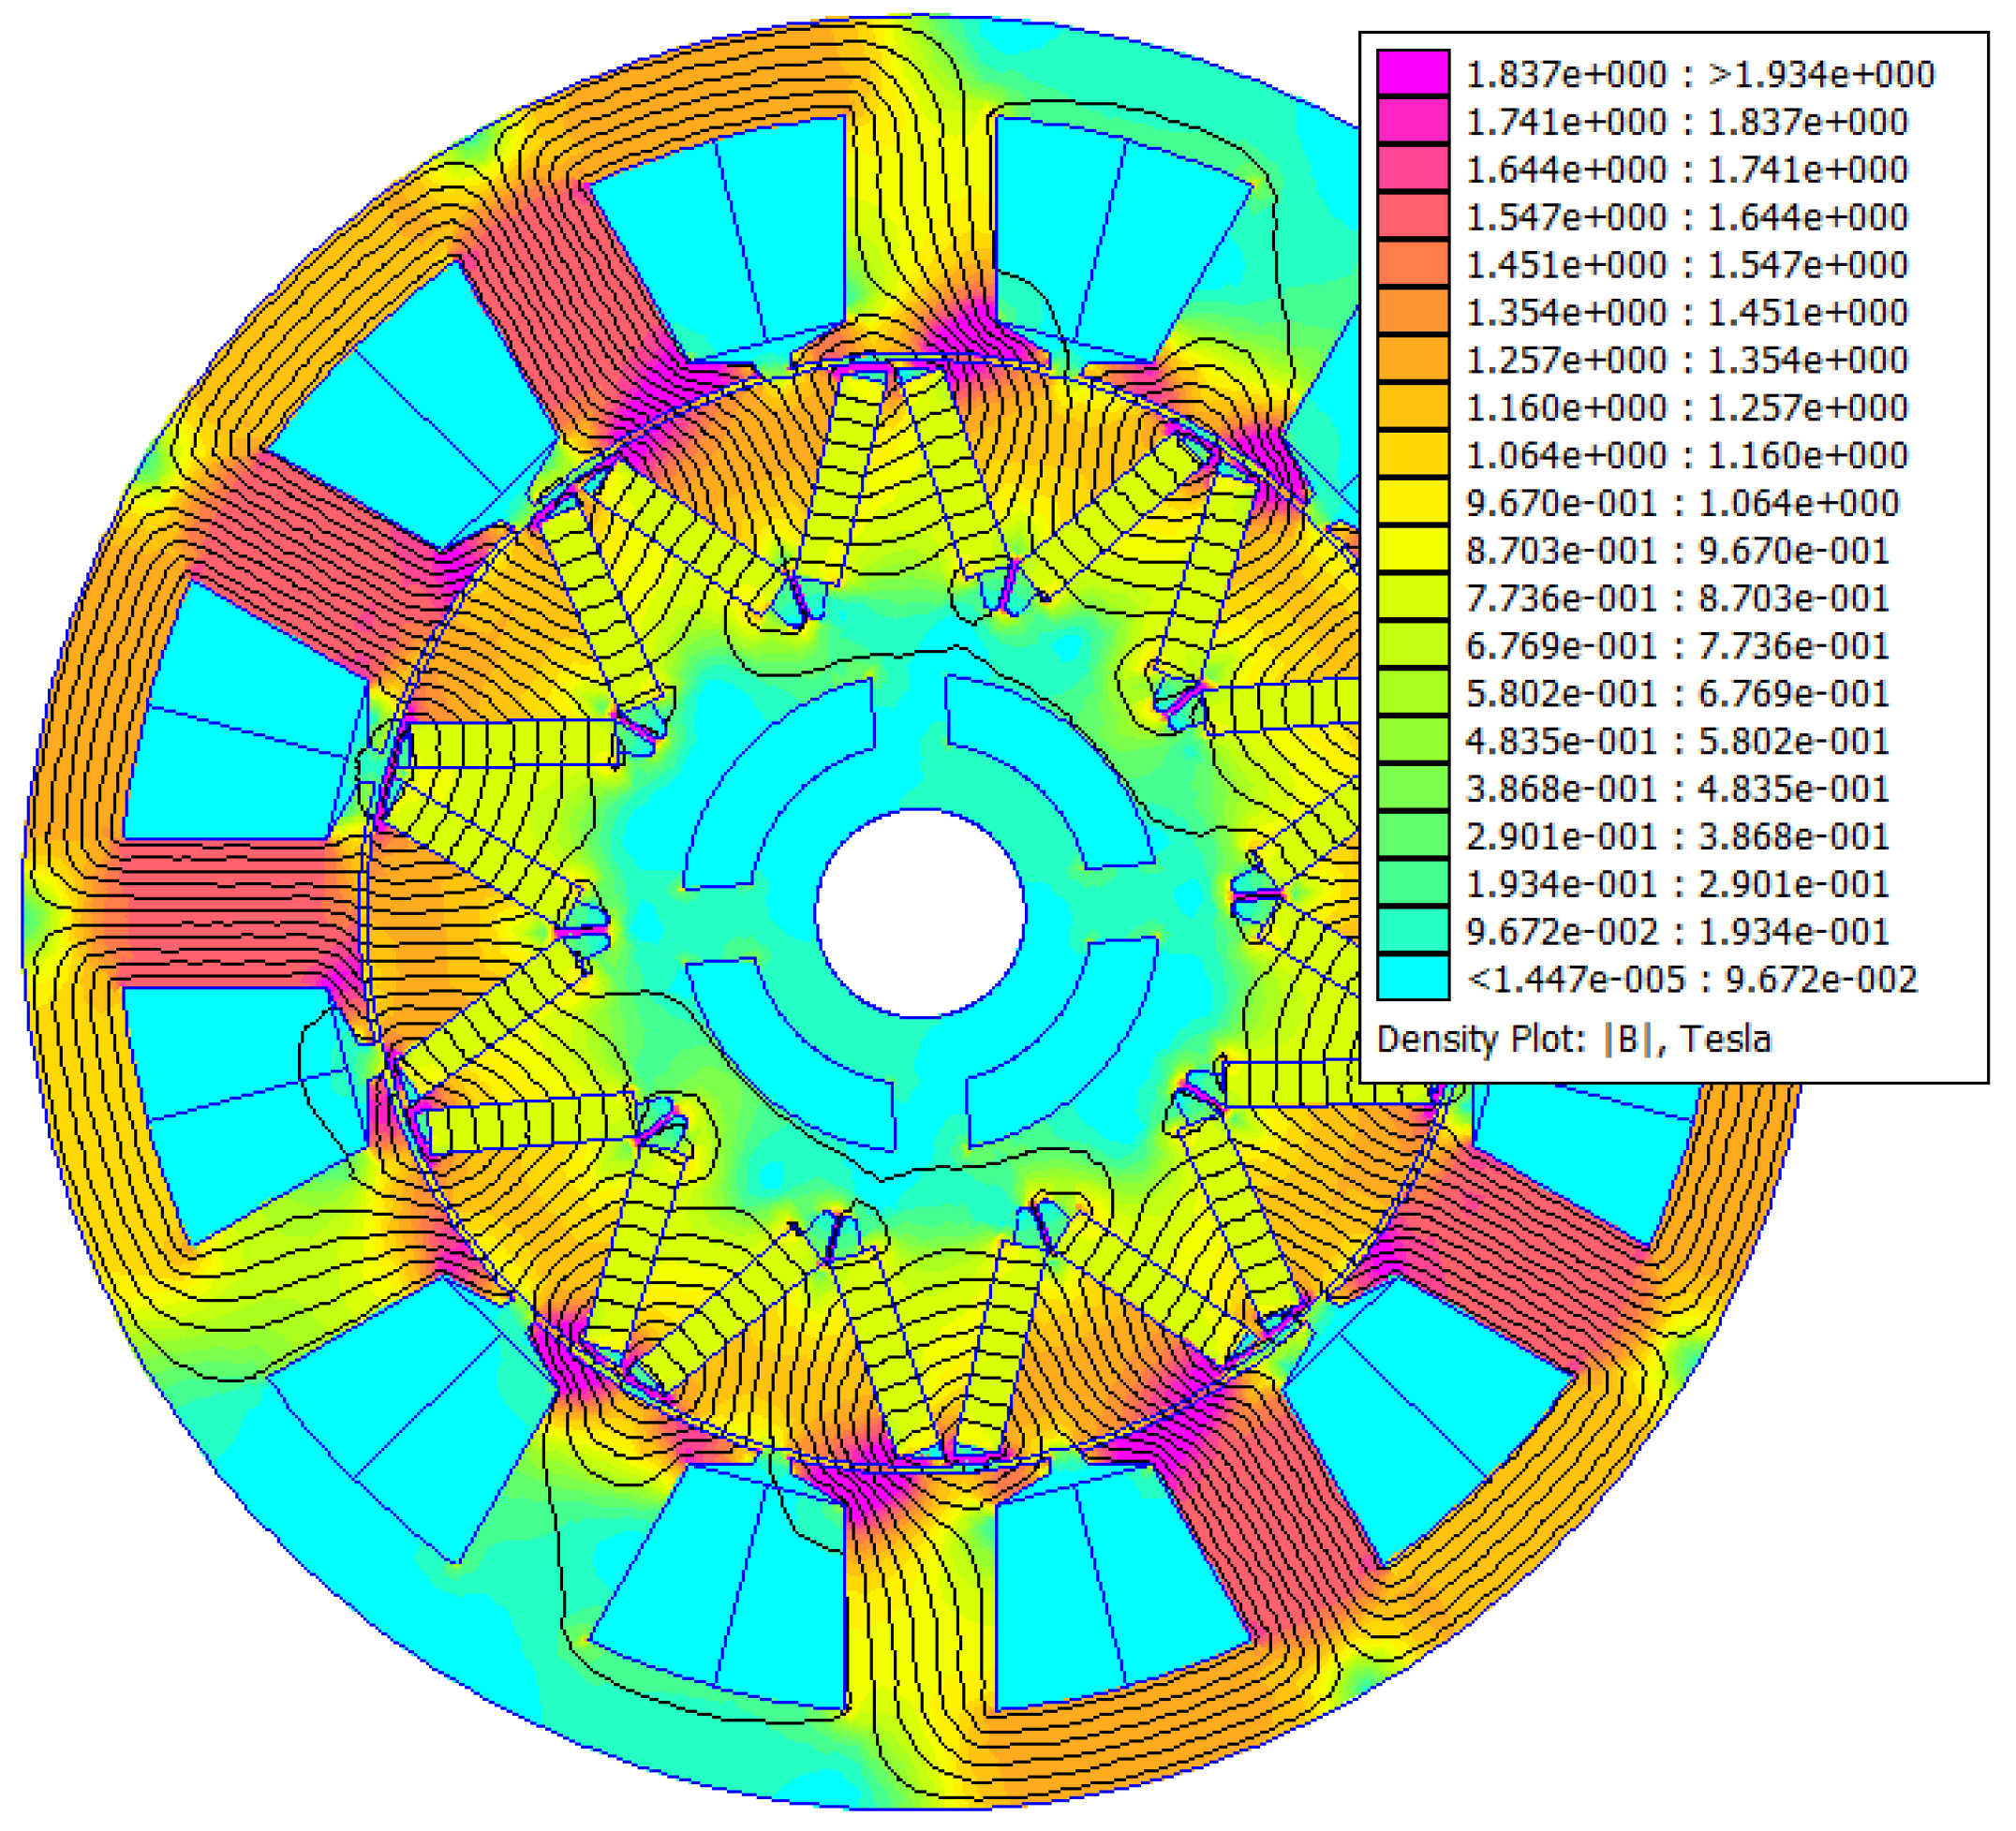
\includegraphics[height=0.75\textheight]{fig/lec03/IPMSM_flux_density_example.png}
        \caption{Exemplary cross-section of an IPMSM with flux density distribution (source: \href{https://www.mdpi.com/2076-3417/12/23/11956}{10.3390/app122311956}, \href{https://creativecommons.org/licenses/by/4.0/deed.en}{CC BY 4.0})}
        \label{fig:motor_cross_section}
    \end{figure}
\end{frame}

%%%%%%%%%%%%%%%%%%%%%%%%%%%%%%%%%%%%%%%%%%%%%%%%%%%%%%%%%%%%%
%% Flux saturation in electric machines (cont.) %%
%%%%%%%%%%%%%%%%%%%%%%%%%%%%%%%%%%%%%%%%%%%%%%%%%%%%%%%%%%%%%
\begin{frame}
    \frametitle{Flux saturation in electric machines (cont.)}
    \begin{figure}
        \centering
        \movie[height=0.74\textheight]{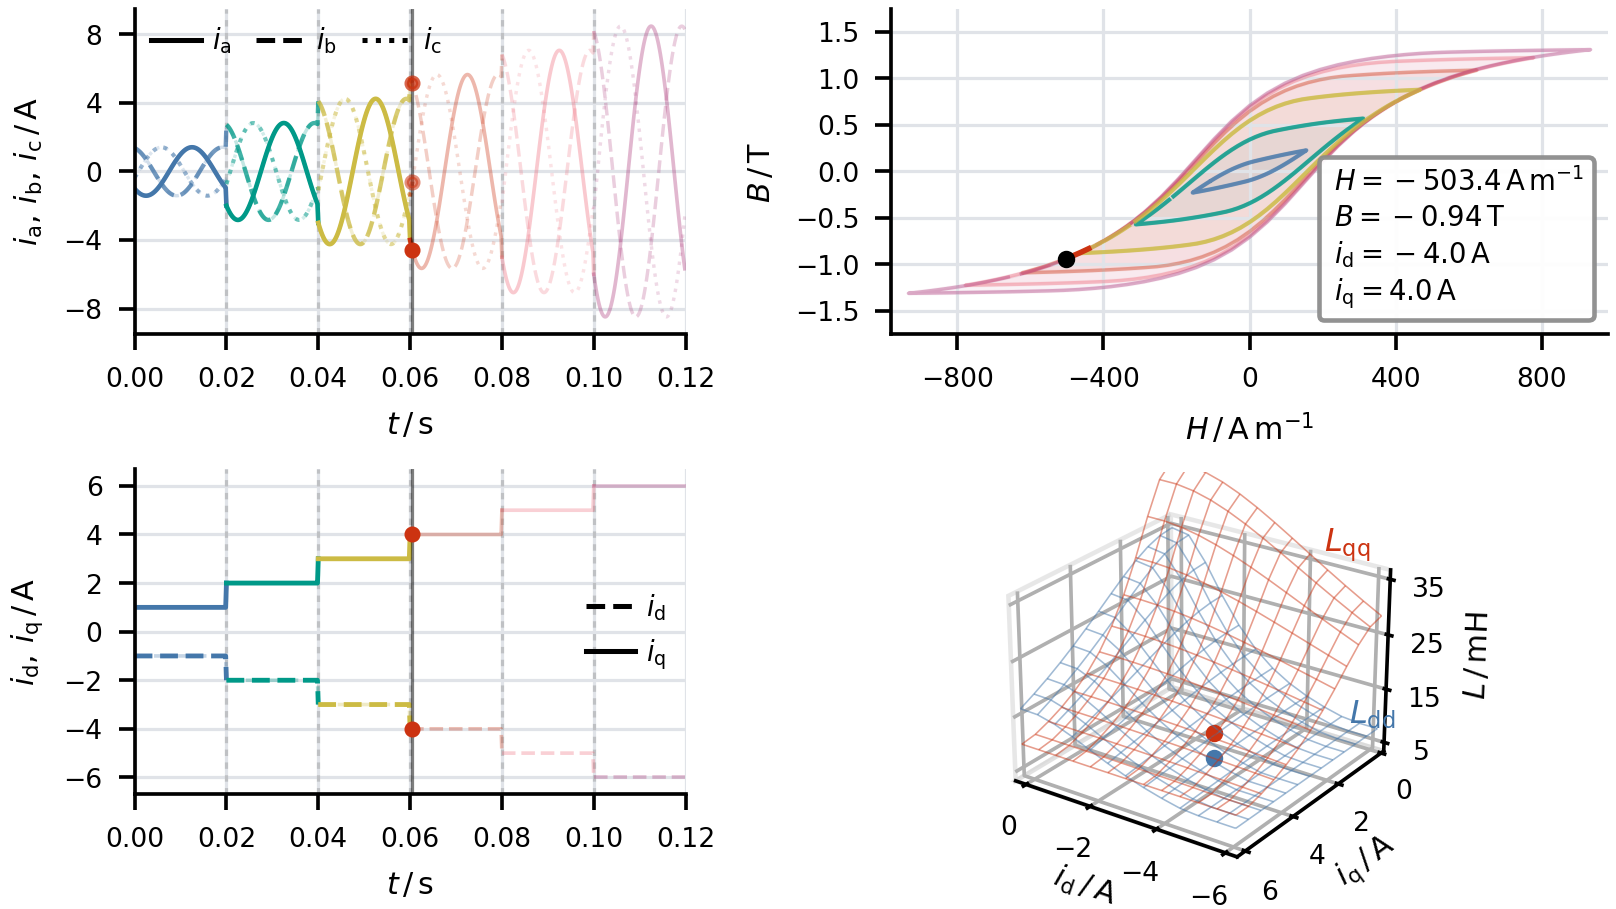
\includegraphics[height=0.678\textheight]{fig/lec03/PMSM_Saturation_BH_Example.png}}{fig/lec03/PMSM_Saturation_BH_Example.mp4}
        \caption{Illustrative and simplified representation of flux saturation in a PMSM based on the \href{https://en.wikipedia.org/wiki/Jiles\%E2\%80\%93Atherton_model}{Jiles-Atherton} B-H curve model (animation)}
        \label{fig:pmsm_saturation_bh_animation}
    \end{figure}
\end{frame}

%%%%%%%%%%%%%%%%%%%%%%%%%%%%%%%%%%%%%%%%%%%%%%%%%%%%%%%%%%%%%
%% Flux saturation: apparent vs.\ differential inductance %%
%%%%%%%%%%%%%%%%%%%%%%%%%%%%%%%%%%%%%%%%%%%%%%%%%%%%%%%%%%%%%
\begin{frame}
    \frametitle{Flux linkage saturation: apparent vs.\ differential inductance}
    \begin{figure}
        \centering
        \begin{tikzpicture}
            \begin{axis}[
                    width=0.72\textwidth,
                    height=0.62\textheight,
                    xlabel={$i$},
                    ylabel={$\psi,\,  L,\,  L_{\mathrm{app}}$},
                    xmin=-0.3, xmax=10.8,
                    ymin=-0.08, ymax=3.40,
                    axis lines=left,
                    clip=false,
                    xtick=\empty,
                    ytick=\empty,
                    xlabel style = {at={(axis description cs:1,0)},anchor=north east},
                    ylabel style = {at={(axis description cs:0,1)},anchor=south east},
                    legend style={at={(1.02,0.98)}, anchor=north west,
                            draw=black, fill=white, font=\small,
                            legend cell align=left,
                            inner xsep=6pt, inner ysep=4pt},
                ]
                %-- Flux saturation curve: psi(i) = 3*tanh(i/3) --%
                \addplot[black, very thick, smooth, domain=0:10.4, samples=120]
                {3*tanh(x/3)};
                \addlegendentry{$\psi$}

                %-- Differential inductance: L = d(psi)/di = 1/cosh^2(i/3) --%

                \addplot[signalalpha, thick, smooth, domain=0.01:10.4, samples=120, visible on=<3->]
                {1/(cosh(x/3)^2)};
                \addlegendentry[visible on=<3->]{$L = \nicefrac{\mathrm{d}\psi}{\mathrm{d}i}$}

                %-- Apparent inductance: L_app = psi/i = 3/i * tanh(i/3) --%

                \addplot[signaldelta, thick, smooth, domain=0.10:10.4, samples=120, visible on=<2->]
                {3/x * tanh(x/3)};
                \addlegendentry[visible on=<2->]{$L_{\mathrm{app}} = \nicefrac{\psi}{i}$}

                %-- Tangent lines at operating points (signalalpha, dashed) --%

                % i1=1.5: psi1=3*tanh(0.5)=1.3863, L1=1/cosh(0.5)^2=0.7864
                \addplot[signalalpha, dashed, thick, domain=0:3.2, forget plot, visible on=<3->]
                {0.7864*(x-1.5) + 1.3863};
                % i2=4: psi2=3*tanh(4/3)=2.6141, L2=1/cosh(4/3)^2=0.2604
                \addplot[signalalpha, dashed, thick, domain=1.3:6.5, forget plot, visible on=<3->]
                {0.2604*(x-4) + 2.6141};
                % i3=7: psi3=3*tanh(7/3)=2.9447, L3=1/cosh(7/3)^2=0.0387
                \addplot[signalalpha, dashed, thick, domain=4.8:9.2, forget plot, visible on=<3->]
                {0.0387*(x-7) + 2.9447};

                %-- Secant lines from origin (signaldelta, dotted) --%

                % L_app1 = 1.3863/1.5 = 0.9242
                \addplot[signaldelta, dotted, thick, domain=0:2.0, forget plot, visible on=<2->]
                {0.9242*x};
                % L_app2 = 2.6141/4 = 0.6535
                \addplot[signaldelta, dotted, thick, domain=0:4.8, forget plot, visible on=<2->]
                {0.6535*x};
                % L_app3 = 2.9447/7 = 0.4207
                \addplot[signaldelta, dotted, thick, domain=0:7.8, forget plot, visible on=<2->]
                {0.4207*x};

                %-- Operating points --%
                \addplot[black, mark=*, mark size=2.5pt, only marks, forget plot]
                coordinates {(1.5, 1.3863) (4, 2.6141) (7, 2.9447)};

                %-- Operating point labels --%
                \node[above left, font=\small] at (axis cs:1.5, 1.3863)
                {$(i_1,\psi_1)$};
                \node[above left, font=\small] at (axis cs:4, 2.6141)
                {$(i_2,\psi_2)$};
                \node[above, font=\small] at (axis cs:7, 2.9447)
                {$(i_3,\psi_3)$};
            \end{axis}
        \end{tikzpicture}
        \caption{Nonlinear flux linkage $\psi(i)$ with the differential inductance $L$ (slope of the tangent) and the apparent inductance $L_{\mathrm{app}}$ (slope of the secant from the origin) -- inspired by \href{https://www.researchgate.net/publication/384459015_A_generic_approach_to_modern_electrical_drives_Tutorial_at_PEMC_2024}{10.13140/RG.2.2.33279.01443}}
        \label{fig:flux_saturation}
    \end{figure}
\end{frame}

%%%%%%%%%%%%%%%%%%%%%%%%%%%%%%%%%%%%%%%%%%%%%%%%%%%%%%%%%%%%%
%% PMSM current-to-flux maps   %%
%%%%%%%%%%%%%%%%%%%%%%%%%%%%%%%%%%%%%%%%%%%%%%%%%%%%%%%%%%%%%
\begin{frame}
    \frametitle{PMSM current-to-flux maps: nonlinear magnetic saturation}

    \begin{figure}
        \begin{tikzpicture}
            \begin{groupplot}[
                    group style={group size=2 by 1, horizontal sep=2.5cm},
                    width=7cm,
                    height=6.25cm,
                    view={-45}{24},
                    xlabel={$i_{\mathrm{d}}\,/\,\mathrm{A}$},
                    ylabel={$i_{\mathrm{q}}\,/\,\mathrm{A}$},
                    xmin=-250, xmax=0,
                    ymin=-250, ymax=250,
                    enlargelimits=false,
                    xlabel style={yshift=2ex},
                    ylabel style={yshift=2ex},
                    xtick={-200,-100,0},
                    ytick={-200,-100, 0,100,200},
                    grid=major,
                    grid style={line width=.1pt, draw=gray!40},
                    tick label style={font=\small},
                    label style={font=\normalsize},
                    zlabel style={font=\normalsize},
                    title style={font=\normalsize},
                ]
                \nextgroupplot[
                    zlabel={$\psi_{\mathrm{d}}\,/\,\mathrm{mVs}$},
                    ztick={0, 25, 50},
                ]
                \addplot3[
                    surf,
                    mesh/rows=26,
                    mesh/cols=14,
                    draw=black,
                    shader=flat,
                    fill=signalalpha,
                    opacity=0.78,
                ]
                table[x=id,y=iq,z expr=1000*\thisrow{psi_d}] {fig/lec03/PMSM_flux_maps.dat};

                \nextgroupplot[
                    zlabel={$\psi_{\mathrm{q}}\,/\,\mathrm{mVs}$},
                ]
                \addplot3[
                    surf,
                    mesh/rows=26,
                    mesh/cols=14,
                    draw=black,
                    shader=flat,
                    fill=signalalpha,
                    opacity=0.78,
                ]
                table[x=id,y=iq,z expr=1000*\thisrow{psi_q}] {fig/lec03/PMSM_flux_maps.dat};
            \end{groupplot}
        \end{tikzpicture}
        \caption{Exemplary current-to-flux maps for a \SI{68}{\kilo\watt} PMSM (derived from \href{https://ieeexplore.ieee.org/document/10098161}{10.1109/TPEL.2023.3265705}, \href{https://creativecommons.org/licenses/by/4.0/deed.en}{CC BY 4.0})}
        \label{fig:flux_maps_BRUSA}
    \end{figure}
\end{frame}

%%%%%%%%%%%%%%%%%%%%%%%%%%%%%%%%%%%%%%%%%%%%%%%%%%%%%%%%%%%%%
%% PMSM current-to-flux maps (cont.): differential inductances   %%
%%%%%%%%%%%%%%%%%%%%%%%%%%%%%%%%%%%%%%%%%%%%%%%%%%%%%%%%%%%%%
\begin{frame}
    \frametitle{PMSM current-to-flux maps (cont.): differential inductances}
    \begin{figure}
        \begin{tikzpicture}
            \begin{groupplot}[
                    group style={group size=2 by 2, horizontal sep=2.55cm, vertical sep=0.6cm},
                    width=0.4\textwidth,
                    height=0.285\textwidth,
                    xlabel={$i_\mathrm{d} / \mathrm{A}$},
                    ylabel={$i_\mathrm{q} / \mathrm{A}$},
                    xmin=-250, xmax=0,
                    ymin=-250, ymax=250,
                    xlabel style={yshift=2ex},
                    ylabel style={yshift=2ex},
                    view={-45}{40},
                    enlargelimits=false,
                    grid=major,
                    grid style={line width=.1pt, draw=gray!40},
                    minor tick num=1,
                    tick label style={font=\small},
                    label style={font=\small},
                    title style={font=\small},
                ]
                \nextgroupplot[
                    zlabel={$L_\mathrm{dd}/ \mathrm{mH}$}
                ]
                \addplot3[surf,
                    mesh/rows=26,
                    mesh/cols=14,
                    shader=flat,
                    draw=black,
                    fill=signalalpha,
                    opacity=0.78,]
                table[x=id, y=iq, z expr=1000*\thisrow{L_dd}] {fig/lec03/PMSM_diff_inductance_maps.dat};

                \nextgroupplot[
                    zlabel={$L_\mathrm{dq} / \mathrm{mH}$}
                ]
                \addplot3[surf,
                    mesh/rows=26,
                    mesh/cols=14,
                    shader=flat,
                    draw=black,
                    fill=signalalpha,
                    opacity=0.78,]
                table[x=id, y=iq, z expr=1000*\thisrow{L_dq}] {fig/lec03/PMSM_diff_inductance_maps.dat};
                \nextgroupplot[
                    zlabel={$L_\mathrm{qd}/ \mathrm{mH}$},
                ]
                \addplot3[surf,
                    mesh/rows=26,
                    mesh/cols=14,
                    shader=flat,
                    draw=black,
                    fill=signalalpha,
                    opacity=0.78,]
                table[x=id, y=iq, z expr=1000*\thisrow{L_qd}] {fig/lec03/PMSM_diff_inductance_maps.dat};

                \nextgroupplot[
                    zlabel={$L_\mathrm{qq}/ \mathrm{mH}$},
                ]
                \addplot3[surf,
                    mesh/rows=26,
                    mesh/cols=14,
                    shader=flat,
                    draw=black,
                    fill=signalalpha,
                    opacity=0.78,]
                table[x=id, y=iq, z expr=1000*\thisrow{L_qq}] {fig/lec03/PMSM_diff_inductance_maps.dat};
            \end{groupplot}
        \end{tikzpicture}
        \caption{Exemplary differential inductance maps derived from \figref{fig:flux_maps_BRUSA}}
        \label{fig:inductance_maps_BRUSA}
    \end{figure}
\end{frame}







%%%%%%%%%%%%%%%%%%%%%%%%%%%%%%%%%%%%%%%%%%%%%%%%%%%%%%%%%%%%%
%% Nonlinear PMSM flux linkage model and inductances %%
%%%%%%%%%%%%%%%%%%%%%%%%%%%%%%%%%%%%%%%%%%%%%%%%%%%%%%%%%%%%%
\begin{frame}
    \frametitle{Nonlinear PMSM flux linkage model and inductances}
    Consider the following nonlinear flux linkage model in dq coordinates for a PMSM:
    \begin{equation}
        \bm{\psi}_\mathrm{s,dq}(t) = \begin{bmatrix}
            \psi_\mathrm{s,d}(t) \\
            \psi_\mathrm{s,q}(t)
        \end{bmatrix} = \bm{f}_{\psi_\mathrm{s}}(\bm{i}_\mathrm{s,dq}(t)).
        \label{eq:nonlinear_flux_function_PMSM}
    \end{equation}
    \onslide<2->{Applying the chain rule yields the time derivative}
    \begin{equation}
        \begin{split}
            \onslide<2->{\frac{\mathrm{d}}{\mathrm{d}t}\bm{\psi}_\mathrm{s,dq}(t)
                               = \underbrace{\frac{\partial \bm{f}_{\psi_\mathrm{s}}}{\partial \bm{i}_\mathrm{s,dq}}}_{\displaystyle=\,\bm{L}(\bm{i}_\mathrm{s,dq})}
                               \frac{\mathrm{d}}{\mathrm{d}t}\bm{i}_\mathrm{s,dq}(t) &} \onslide<3->{= \begin{bmatrix}
                                                                                                               \text{\makebox[\widthof{$L_\mathrm{dd}(\bm{i}_\mathrm{s,dq})$}][c]{$\dfrac{\partial \psi_\mathrm{s,d}}{\partial i_\mathrm{s,d}}$}} &
                                                                                                               \text{\makebox[\widthof{$L_\mathrm{dq}(\bm{i}_\mathrm{s,dq})$}][c]{$\dfrac{\partial \psi_\mathrm{s,d}}{\partial i_\mathrm{s,q}}$}}   \\[1.5ex]
                                                                                                               \text{\makebox[\widthof{$L_\mathrm{qd}(\bm{i}_\mathrm{s,dq})$}][c]{$\dfrac{\partial \psi_\mathrm{s,q}}{\partial i_\mathrm{s,d}}$}} &
                                                                                                               \text{\makebox[\widthof{$L_\mathrm{qq}(\bm{i}_\mathrm{s,dq})$}][c]{$\dfrac{\partial \psi_\mathrm{s,q}}{\partial i_\mathrm{s,q}}$}}
                                                                                                           \end{bmatrix}\frac{\mathrm{d}}{\mathrm{d}t}\bm{i}_\mathrm{s,dq}(t)} \\ & \onslide<4->{= \begin{bmatrix}
                                                                                                                                                                                                           L_\mathrm{dd}(\bm{i}_\mathrm{s,dq}) & L_\mathrm{dq}(\bm{i}_\mathrm{s,dq}) \\[1.6ex]
                                                                                                                                                                                                           L_\mathrm{qd}(\bm{i}_\mathrm{s,dq}) & L_\mathrm{qq}(\bm{i}_\mathrm{s,dq})
                                                                                                                                                                                                       \end{bmatrix}\frac{\mathrm{d}}{\mathrm{d}t}\bm{i}_\mathrm{s,dq}(t),}
        \end{split}
    \end{equation}
    \onslide<4->{where the \hl{differential inductance matrix} $\bm{L}(\bm{i}_\mathrm{s,dq})$ is the Jacobian of $\bm{f}_{\psi_\mathrm{s}}$ with respect to $\bm{i}_\mathrm{s,dq}$.}
\end{frame}

%%%%%%%%%%%%%%%%%%%%%%%%%%%%%%%%%%%%%%%%%%%%%%%%%%%%%%%%%%%%%
%% Nonlinear PMSM flux linkage model and inductances (cont) %%
%%%%%%%%%%%%%%%%%%%%%%%%%%%%%%%%%%%%%%%%%%%%%%%%%%%%%%%%%%%%%
\begin{frame}
    \frametitle{Nonlinear PMSM flux linkage model and inductances (cont.)}
    Representing the nonlinear flux linkage model \eqref{eq:nonlinear_flux_function_PMSM} based on the \hl{apparent inductance matrix} $\bm{L}_{\mathrm{app}}(\bm{i}_\mathrm{s,dq})$ yields
    \begin{equation}
        \bm{\psi}_\mathrm{s,dq}(t) = \bm{L}_{\mathrm{app}}(\bm{i}_\mathrm{s,dq}(t))\bm{i}_\mathrm{s,dq}(t) + \bm{\psi}_\mathrm{PM}
    \end{equation}\pause
    with
    \begin{equation}
        \bm{L}_{\mathrm{app}}(\bm{i}_\mathrm{s,dq}) = \begin{bmatrix}
            L_{\mathrm{dd,app}}(i_\mathrm{s,d})                 & L_{\mathrm{dq,app}}(i_\mathrm{s,d}, i_\mathrm{s,q}) \\[1.5ex]
            L_{\mathrm{qd,app}}(i_\mathrm{s,d}, i_\mathrm{s,q}) & L_{\mathrm{qq,app}}(i_\mathrm{s,q})
        \end{bmatrix}, \quad \bm{\psi}_\mathrm{PM} = \begin{bmatrix}
            \psi_\mathrm{PM} \\[1.5ex]
            0
        \end{bmatrix}.
    \end{equation}\pause
    Here, the following can be noted:
    \begin{itemize}
        \item Main diagonal elements of $\bm{L}_{\mathrm{app}}$ depend only on the respective current component since otherwise the current-to-flux maps would be not unique (overdetermined system).\pause
        \item Since the apparent inductance matrix represents the absolute flux linkage change due to the stator currents, the PM flux linkage $\bm{\psi}_\mathrm{PM}$ is explicitly included in the model.\pause
        \item Since the apparent inductance representation is less elegant than the original flux function $\bm{f}_{\psi_\mathrm{s}}$ and partly ambiguous, it is not commonly used for control-oriented modeling of PMSMs.
    \end{itemize}
\end{frame}

%%%%%%%%%%%%%%%%%%%%%%%%%%%%%%%%%%%%%%%%%%%%%%%%%%%%%%%%%%%%%
%% Current differential equations of the nonlinear PMSM model %%
%%%%%%%%%%%%%%%%%%%%%%%%%%%%%%%%%%%%%%%%%%%%%%%%%%%%%%%%%%%%%
\begin{frame}
    \frametitle{Current differential equations of the nonlinear PMSM model}
    Utilizing the differential inductance concept, the \hl{current differential equation} can be derived as
    \begin{equation}
        \begin{split}
            \bm{u}_\mathrm{s,dq}(t) & = R_\mathrm{s} \bm{i}_\mathrm{s,dq}(t)+ \omega(t)\bm{J}\bm{\psi}_\mathrm{s,dq}(t) + \nicefrac{\mathrm{d}}{\mathrm{d}t}\bm{\psi}_\mathrm{s,dq}(t) \\ \onslide<2->{&= R_\mathrm{s} \bm{i}_\mathrm{s,dq}(t)+ \omega(t)\bm{J}\bm{f}_{\psi_\mathrm{s}}(\bm{i}_\mathrm{s,dq}(t)) + \bm{L}(\bm{i}_\mathrm{s,dq})\frac{\mathrm{d}}{\mathrm{d}t}\bm{i}_\mathrm{s,dq}(t)} \\
            \onslide<3->{\Leftrightarrow  \frac{\mathrm{d}}{\mathrm{d}t}\bm{i}_\mathrm{s,dq}(t) & = \bm{L}^{-1}(\bm{i}_\mathrm{s,dq})\left[\bm{u}_\mathrm{s,dq}(t)- R_\mathrm{s} \bm{i}_\mathrm{s,dq}(t)- \omega(t)\bm{J}\bm{f}_{\psi_\mathrm{s}}(\bm{i}_\mathrm{s,dq}(t))\right].}
        \end{split}
    \end{equation}
    \begin{itemize}
        \item<4-> The model $\bm{f}_{\psi_\mathrm{s}}$ can be implemented as look-up table (LUT) plus interpolation or as a function approximator (e.g., neural network, polynomial, prototype functions).
        \item<5-> Inverse $\bm{L}^{-1}(\bm{i}_\mathrm{s,dq})$ can be precomputed offline based on finite difference or analytical differentiation depending on the implementation of $\bm{f}_{\psi_\mathrm{s}}$.
        \item<6-> Alternatively, one can integrate the flux ODE \eqref{eq:basic_PMSM_model_set} and then compute  $\bm{i}_\mathrm{s,dq}=\bm{f}_{\psi_\mathrm{s}}^{-1}(\bm{\psi}_\mathrm{s,dq})$.
    \end{itemize}
\end{frame}

%%%%%%%%%%%%%%%%%%%%%%%%%%%%%%%%%%%%%%%%%%%%%%%%%%%%%%%%%%%%%
%% Current differential equations of the nonlinear PMSM model %%
%%%%%%%%%%%%%%%%%%%%%%%%%%%%%%%%%%%%%%%%%%%%%%%%%%%%%%%%%%%%%
\begin{frame}
    \frametitle{Linear PMSM model with constant inductances}
    Applying the \hl{first-order Taylor expansion} to the nonlinear flux function $\bm{f}_{\psi_\mathrm{s}}$ around some operating point (typically the origin $\bm{i}_\mathrm{s,dq}=\bm{0}$) yields the \hl{linear PMSM flux model}
    \begin{equation}
        \bm{\psi}_\mathrm{s,dq}(t)  \approx \underbrace{\bm{f}_{\psi_\mathrm{s}}(\bm{0})\vphantom{\frac{\partial \bm{f}_{\psi_\mathrm{s}}}{\partial \bm{i}_\mathrm{s,dq}}\bigg|_{\bm{i}_\mathrm{s,dq}=\bm{0}}}}_{\displaystyle=\bm{\psi}_\mathrm{PM}} + \underbrace{\frac{\partial \bm{f}_{\psi_\mathrm{s}}}{\partial \bm{i}_\mathrm{s,dq}}\bigg|_{\bm{i}_\mathrm{s,dq}=\bm{0}}}_{\displaystyle=\,\bm{L}_0}\bm{i}_\mathrm{s,dq}(t)  \onslide<2->{= \begin{bmatrix}
                    \psi_{\mathrm{PM}} \\
                    0
                \end{bmatrix} + \begin{bmatrix}
                    L_{\mathrm{dd},0} & L_{\mathrm{dq},0} \\
                    L_{\mathrm{qd},0} & L_{\mathrm{qq},0}
                \end{bmatrix}\bm{i}_\mathrm{s,dq}(t)}.
    \end{equation}
    \onslide<3->{With this linear flux model, the current ODE simplifies to}
    \begin{equation}
        \begin{split}
            \onslide<3->{\bm{u}_\mathrm{s,dq}(t)                                                & = R_\mathrm{s} \bm{i}_\mathrm{s,dq}(t)+ \omega(t)\bm{J}\left[\bm{\psi}_\mathrm{PM} + \bm{L}_0 \bm{i}_\mathrm{s,dq}(t)\right] + \bm{L}_0\frac{\mathrm{d}}{\mathrm{d}t}\bm{i}_\mathrm{s,dq}(t)} \\
            \onslide<4->{\Leftrightarrow  \frac{\mathrm{d}}{\mathrm{d}t}\bm{i}_\mathrm{s,dq}(t) & = \bm{L}_0^{-1}\left[\bm{u}_\mathrm{s,dq}(t)- R_\mathrm{s} \bm{i}_\mathrm{s,dq}(t)- \omega(t)\bm{J}\left(\bm{\psi}_\mathrm{PM} + \bm{L}_0 \bm{i}_\mathrm{s,dq}(t)\right)\right].}
        \end{split}
    \end{equation}
    \onslide<5->{And the torque expressions results in
            \begin{equation}
                T(t) = \frac{3}{2}p\left[\psi_\mathrm{PM} i_\mathrm{s,q}(t) + (L_{\mathrm{dd},0}-L_{\mathrm{qq},0})i_\mathrm{s,d}(t)i_\mathrm{s,q}(t) + L_{\mathrm{dq},0} i_\mathrm{s,d}^2(t) - L_{\mathrm{qd},0} i_\mathrm{s,q}^2(t)\right].
            \end{equation}}
\end{frame}

%%%%%%%%%%%%%%%%%%%%%%%%%%%%%%%%%%%%%%%%%%%%%%%%%%%%%%%%%%%%%
%% Current differential equations of the nonlinear PMSM model %%
%%%%%%%%%%%%%%%%%%%%%%%%%%%%%%%%%%%%%%%%%%%%%%%%%%%%%%%%%%%%%
\begin{frame}
    \frametitle{Linear PMSM model with constant inductances (cont.)}
    As can be seen from \figref{fig:inductance_maps_BRUSA} the off-diagonal inductance terms $L_{\mathrm{dq},0}$ and $L_{\mathrm{qd},0}$ are much smaller than the main diagonal terms $L_{\mathrm{dd},0}$ and $L_{\mathrm{qq},0}$. \pause Thus, by further simplification
    $$
        L_{\mathrm{dq},0} \approx L_{\mathrm{qd},0} \approx 0
    $$\pause
    we obtain the following current ODE
    \begin{equation}
        \frac{\mathrm{d}}{\mathrm{d}t}\bm{i}_\mathrm{s,dq}(t) = \begin{bmatrix}
            L_{\mathrm{dd},0}^{-1} & 0                      \\
            0                      & L_{\mathrm{qq},0}^{-1}
        \end{bmatrix}\left[\bm{u}_\mathrm{s,dq}(t)- R_\mathrm{s} \bm{i}_\mathrm{s,dq}(t)- \omega(t)\bm{J}\left(\bm{\psi}_\mathrm{PM} + \begin{bmatrix}
                L_{\mathrm{dd},0} & 0                 \\
                0                 & L_{\mathrm{qq},0}
            \end{bmatrix} \bm{i}_\mathrm{s,dq}(t)\right)\right].
    \end{equation}\pause
    and torque expression
    \begin{equation}
        T(t) = \frac{3}{2}p\left[\psi_\mathrm{PM} i_\mathrm{s,q}(t) + (L_{\mathrm{dd},0}-L_{\mathrm{qq},0})i_\mathrm{s,d}(t)i_\mathrm{s,q}(t)\right].
    \end{equation}\pause
    This is the \hl{standard linear model for IPMSMs} with constant inductances. For \hl{SPMSMs}, there is no \hl{magnetic anistropy} in the dq-paths, i.e., $L_{\mathrm{dd},0} \approx L_{\mathrm{qq},0}$ and the torque expression further simplifies to $T(t) = \frac{3}{2}p\psi_\mathrm{PM} i_\mathrm{s,q}(t)$.
\end{frame}

%%%%%%%%%%%%%%%%%%%%%%%%%%%%%%%%%%%%%%%%%%%%%%%%%%%%%%%%%%%%%
%% Flux linkage harmonics %%
%%%%%%%%%%%%%%%%%%%%%%%%%%%%%%%%%%%%%%%%%%%%%%%%%%%%%%%%%%%%%
\begin{frame}
    \frametitle{Flux linkage harmonics}
    The model \eqref{eq:basic_PMSM_model_set} is called the \hl{fundamental wave model} since it only considers the fundamental spatial harmonic of the flux linkage distribution. \onslide<2->{However, in a real machine multiple rotor angle-dependent effects shape the flux linkage distribution:}
    \begin{itemize}
        \item<2-> Design: slot and winding distribution impacts, motor skew along the axial direction, etc.,
        \item<3-> Production: geometry and material tolerances, assembly inaccuracies, etc.
    \end{itemize}
    \begin{figure}
        \begin{tikzpicture}
            \begin{groupplot}[
                    group style={group size=2 by 1, horizontal sep=2.4cm},
                    width=0.43\textwidth,
                    height=0.26\textwidth,
                    xmin=0, xmax=360,
                    xtick={0,90,180,270,360},
                    xlabel={$\varepsilon\,/\,^\circ$},
                    grid=major,
                    grid style={line width=.1pt, draw=gray!40},
                    tick label style={font=\small},
                    label style={font=\normalsize},
                    title style={font=\normalsize},
                    enlargelimits=false,
                ]
                \nextgroupplot[
                    ylabel={$\psi_\mathrm{d}\,/\,\mathrm{mVs}$},
                    ymin=32, ymax=44,
                    ytick={32,35,38,41,44},
                ]
                \addplot[
                    signalalpha,
                    very thick,
                ]
                table[x=Angle_el, y expr=1000*\thisrow{Psi_d}, col sep=comma] {fig/lec03/Harmonics_PMSM.csv};

                \nextgroupplot[
                    ylabel={$\psi_\mathrm{q}\,/\,\mathrm{mVs}$},
                    ymin=-28.5, ymax=-20,
                    ytick={-28,-26,-24,-22,-20},
                ]
                \addplot[
                    signalalpha,
                    very thick,
                ]
                table[x=Angle_el, y expr=1000*\thisrow{Psi_q}, col sep=comma] {fig/lec03/Harmonics_PMSM.csv};
            \end{groupplot}
        \end{tikzpicture}
        \caption{Exemplary  rotor angle $\varepsilon$ dependent flux harmonics of a PMSM for a steady-state operating point (measured at test bench)}
        \label{fig:flux_harmonics_PMSM}
    \end{figure}
\end{frame}

%%%%%%%%%%%%%%%%%%%%%%%%%%%%%%%%%%%%%%%%%%%%%%%%%%%%%%%%%%%%%
%% Flux linkage harmonics %%
%%%%%%%%%%%%%%%%%%%%%%%%%%%%%%%%%%%%%%%%%%%%%%%%%%%%%%%%%%%%%
\begin{frame}
    \frametitle{Flux linkage harmonics (cont.)}
    Considering the above, the flux linkage model becomes rotor angle-dependent:
    \begin{equation}
        \bm{\psi}_\mathrm{s,dq}(t) = \bm{f}_{\psi_\mathrm{s}}(\bm{i}_\mathrm{s,dq}(t), \varepsilon(t)).
    \end{equation}
    \onslide<2->{Consequently, the time derivative of the flux linkage becomes}
    \begin{equation}
        \begin{split}
            \onslide<2->{\frac{\mathrm{d}}{\mathrm{d}t}\bm{\psi}_\mathrm{s,dq}(t) & = \frac{\partial \bm{f}_{\psi_\mathrm{s}}}{\partial \bm{i}_\mathrm{s,dq}}\bigg|_{\varepsilon}\frac{\mathrm{d}}{\mathrm{d}t}\bm{i}_\mathrm{s,dq}(t) + \frac{\partial \bm{f}_{\psi_\mathrm{s}}}{\partial \varepsilon}\bigg|_{\bm{i}_\mathrm{s,dq}}\frac{\mathrm{d}}{\mathrm{d}t}\varepsilon(t)} \\ & \onslide<3->{= \bm{L}(\bm{i}_\mathrm{s,dq}, \varepsilon)\frac{\mathrm{d}}{\mathrm{d}t}\bm{i}_\mathrm{s,dq}(t) + \frac{\partial \bm{f}_{\psi_\mathrm{s}}}{\partial \varepsilon}(\bm{i}_\mathrm{s,dq}, \varepsilon)\omega(t).}
        \end{split}
    \end{equation}
    \onslide<4->{Thus, the flux linkage harmonics introduce an additional induced voltage term into the stator voltage equation:}
    \begin{equation}
        \begin{split}
            \onslide<4->{\bm{u}_\mathrm{s,dq}(t) & = R_\mathrm{s} \bm{i}_\mathrm{s,dq}(t)+ \omega(t)\bm{J}\bm{\psi}_\mathrm{s,dq}(t) + \frac{\mathrm{d}}{\mathrm{d}t}\bm{\psi}_\mathrm{s,dq}(t)} \\ \onslide<5->{& = R_\mathrm{s} \bm{i}_\mathrm{s,dq}(t)+ \omega(t)\bm{J}\bm{f}_{\psi_\mathrm{s}}(\bm{i}_\mathrm{s,dq}(t), \varepsilon(t)) + \bm{L}(\bm{i}_\mathrm{s,dq}, \varepsilon)\frac{\mathrm{d}}{\mathrm{d}t}\bm{i}_\mathrm{s,dq}(t) + \frac{\partial \bm{f}_{\psi_\mathrm{s}}}{\partial \varepsilon}\omega(t).}
        \end{split}
    \end{equation}
\end{frame}



%%%%%%%%%%%%%%%%%%%%%%%%%%%%%%%%%%%%%%%%%%%%%%%%%%%%%%%%%%%%%
%% Synchronous machine (SM) rotor types %%
%%%%%%%%%%%%%%%%%%%%%%%%%%%%%%%%%%%%%%%%%%%%%%%%%%%%%%%%%%%%%
\begin{frame}
    \frametitle{Electrically excited synchronous machine (EESM) rotor types}
    \begin{figure}
        \centering
        \begin{subfigure}{0.49\textwidth}
            \centering
            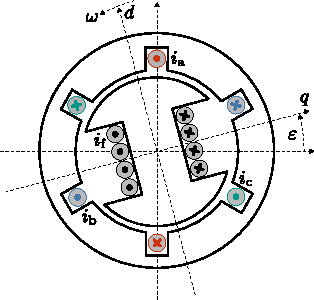
\includegraphics[width=0.8\textwidth]{fig/lec03/SM_salient_pole.pdf}
            \caption{Salient pole rotor}
        \end{subfigure}
        \hfill
        \begin{subfigure}{0.49\textwidth}
            \centering
            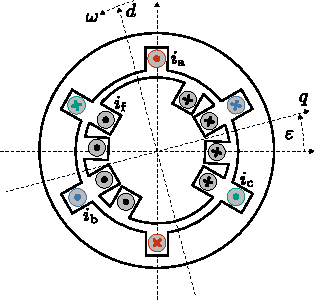
\includegraphics[width=0.8\textwidth]{fig/lec03/SM_cylindrical_rotor.pdf}
            \caption{Cylindrical rotor}
        \end{subfigure}
        \caption{Major rotor types of electrically excited synchronous machines (EESM) with dq reference frame axes aligned to the rotor flux produced by the field winding}
        \label{fig:examples_EESM_rotor}
    \end{figure}
\end{frame}

%%%%%%%%%%%%%%%%%%%%%%%%%%%%%%%%%%%%%%%%%%%%%%%%%%%%%%%%%%%%%
%% Summary: Cylindrical SM model in dq coordinates   %%
%%%%%%%%%%%%%%%%%%%%%%%%%%%%%%%%%%%%%%%%%%%%%%%%%%%%%%%%%%%%%
\begin{frame}
    \frametitle{EESM model in dq coordinates}
    The most important equations of the EESM model in the  dq coordinates are\footnote{A detailed derivation can be found in \href{https://github.com/IAS-Uni-Siegen/EMD_course}{Fundamentals of electrical machines and drives (EMD) course}.}:
    \begin{alignat}{4}
         &  & \text{Stator voltage:} &  & \quad\bm{u}_\mathrm{s,dq}( & t) &  & = R_\mathrm{s} \bm{i}_\mathrm{s,dq}(t)+ \omega(t)\bm{J}\bm{\psi}_\mathrm{s,dq}(t) + \nicefrac{\mathrm{d}}{\mathrm{d}t}\bm{\psi}_\mathrm{s,dq}(t), \notag \\
        \onslide<2->{&  & \text{Rotor / field winding voltage:}      &  & \quad u_\mathrm{f}(            & t) &  & = R_\mathrm{f}i_\mathrm{f}(t)+\nicefrac{\mathrm{d}}{\mathrm{d}t}\psi_\mathrm{f}(t), \notag}                          \\
        \onslide<3->{&  & \text{Stator flux linkage:}                &  & \quad \bm{\psi}_\mathrm{s,dq}( & t) &  & =  \bm{f}_{\psi_\mathrm{s}}(\bm{i}_\mathrm{s,dq}(t), \psi_\mathrm{f}(t)), \label{eq:basic_EESM_model_set}}           \\
        \onslide<4->{&  & \text{Rotor / field winding flux linkage:} &  & \psi_\mathrm{f}(               & t) &  & =  \bm{f}_{\psi_\mathrm{f}}(i_{\mathrm{f}}(t), \bm{i}_\mathrm{s,dq}(t)), \notag}                                     \\
        \onslide<5->{&  & \text{Torque:}                             &  & \quad T(                       & t) &  & = \nicefrac{3}{2} p (\bm{i}_\mathrm{s,dq}(t))\T\bm{J}\bm{\psi}_\mathrm{s,dq}(t) \notag}
    \end{alignat}
    \onslide<6->{with the further signals and parameters:
            \begin{equation*}
                \begin{aligned}
                    \bm{i}_\mathrm{s,dq}: \text{stator current},                                                              &
                    \qquad i_\mathrm{f}  : \text{rotor / field winding current},                                                                                                                                                      \\
                    R_\mathrm{s}:                                                          \text{stator winding resistances}, &
                    \qquad R_\mathrm{f} : \text{rotor / field winding resistance},                                                                                                                                                    \\
                    p                                           : \text{pole pair number},                                    &
                    \qquad \omega = p\omega_\mathrm{me}                   : \text{electrical angular velocity,}                                                                                                                       \\
                    \bm{J}: \text{90° rotation matrix, cf. \eqref{eq:J_rotation}},                                            & \qquad \bm{f}_{\psi_\mathrm{s}}, {f}_{\psi_\mathrm{f}} : \text{stator / rotor flux linkage function}.
                \end{aligned}
            \end{equation*}}
\end{frame}


%%%%%%%%%%%%%%%%%%%%%%%%%%%%%%%%%%%%%%%%%%%%%%%%%%%%%%%%%%%%%
%% EESM current-to-flux maps   %%
%%%%%%%%%%%%%%%%%%%%%%%%%%%%%%%%%%%%%%%%%%%%%%%%%%%%%%%%%%%%%
\begin{frame}
    \frametitle{EESM current-to-flux maps: nonlinear magnetic saturation}

    \begin{figure}
        \begin{tikzpicture}
            \begin{groupplot}[
                    group style={group size=3 by 1, horizontal sep=1.6cm},
                    width=0.32\textwidth,
                    height=0.33\textwidth,
                    view={-45}{24},
                    xlabel={$i_{\mathrm{d}}\,/\,\mathrm{A}$},
                    ylabel={$i_{\mathrm{q}}\,/\,\mathrm{A}$},
                    xmin=-30, xmax=10,
                    ymin=-35, ymax=35,
                    enlargelimits=false,
                    xtick={-30,-15,0,10},
                    ytick={-30,-15,0,15,30},
                    grid=major,
                    grid style={line width=.1pt, draw=gray!40},
                    tick label style={font=\small},
                    label style={font=\normalsize},
                    zlabel style={font=\normalsize},
                    title style={font=\normalsize},
                    xlabel style={yshift=2ex},
                    ylabel style={yshift=2ex},
                ]
                \nextgroupplot[
                    zlabel={$\psi_{\mathrm{d}}\,/\,\mathrm{Vs}$},
                    zmin=-0.50, zmax=1.05,
                ]
                \addplot3[surf, mesh/rows=15, mesh/cols=9, draw=black, shader=flat, fill=signaldelta, opacity=0.78] table[x=id_A,y=iq_A,z=psi_d_Vs_if2,col sep=comma] {fig/lec03/EESM_psi_d.csv};
                \addplot3[surf, mesh/rows=15, mesh/cols=9, draw=black, shader=flat, fill=signalgamma, opacity=0.74] table[x=id_A,y=iq_A,z=psi_d_Vs_if3,col sep=comma] {fig/lec03/EESM_psi_d.csv};
                \addplot3[surf, mesh/rows=15, mesh/cols=9, draw=black, shader=flat, fill=signalbeta, opacity=0.70] table[x=id_A,y=iq_A,z=psi_d_Vs_if4,col sep=comma] {fig/lec03/EESM_psi_d.csv};
                \addplot3[surf, mesh/rows=15, mesh/cols=9, draw=black, shader=flat, fill=signalalpha, opacity=0.66] table[x=id_A,y=iq_A,z=psi_d_Vs_if5,col sep=comma] {fig/lec03/EESM_psi_d.csv};

                \nextgroupplot[
                    zlabel={$\psi_{\mathrm{q}}\,/\,\mathrm{Vs}$},
                    zmin=-1.35, zmax=1.05,
                    zlabel style={yshift=-1ex},
                ]
                \addplot3[surf, mesh/rows=15, mesh/cols=9, draw=black, shader=flat, fill=signaldelta, opacity=0.78] table[x=id_A,y=iq_A,z=psi_q_Vs_if2,col sep=comma] {fig/lec03/EESM_psi_q.csv};
                \addplot3[surf, mesh/rows=15, mesh/cols=9, draw=black, shader=flat, fill=signalgamma, opacity=0.74] table[x=id_A,y=iq_A,z=psi_q_Vs_if3,col sep=comma] {fig/lec03/EESM_psi_q.csv};
                \addplot3[surf, mesh/rows=15, mesh/cols=9, draw=black, shader=flat, fill=signalbeta, opacity=0.70] table[x=id_A,y=iq_A,z=psi_q_Vs_if4,col sep=comma] {fig/lec03/EESM_psi_q.csv};
                \addplot3[surf, mesh/rows=15, mesh/cols=9, draw=black, shader=flat, fill=signalalpha, opacity=0.66] table[x=id_A,y=iq_A,z=psi_q_Vs_if5,col sep=comma] {fig/lec03/EESM_psi_q.csv};

                \nextgroupplot[
                    zlabel={$\psi_{\mathrm{f}}\,/\,\mathrm{Vs}$},
                    zmin=0.24, zmax=1.10,
                    zlabel style={yshift=-1ex},
                ]
                \addplot3[surf, mesh/rows=15, mesh/cols=9, draw=black, shader=flat, fill=signaldelta, opacity=0.78] table[x=id_A,y=iq_A,z=psi_f_Vs_if2,col sep=comma] {fig/lec03/EESM_psi_f.csv};
                \addplot3[surf, mesh/rows=15, mesh/cols=9, draw=black, shader=flat, fill=signalgamma, opacity=0.74] table[x=id_A,y=iq_A,z=psi_f_Vs_if3,col sep=comma] {fig/lec03/EESM_psi_f.csv};
                \addplot3[surf, mesh/rows=15, mesh/cols=9, draw=black, shader=flat, fill=signalbeta, opacity=0.70] table[x=id_A,y=iq_A,z=psi_f_Vs_if4,col sep=comma] {fig/lec03/EESM_psi_f.csv};
                \addplot3[surf, mesh/rows=15, mesh/cols=9, draw=black, shader=flat, fill=signalalpha, opacity=0.66] table[x=id_A,y=iq_A,z=psi_f_Vs_if5,col sep=comma] {fig/lec03/EESM_psi_f.csv};
            \end{groupplot}

            \matrix[matrix of nodes,
                ampersand replacement=\&,
                anchor=south,
                draw=black,
                fill=white,
                inner sep=1.4pt,
                row sep=1pt,
                column sep=5pt,
                nodes={anchor=west, font=\small}]
            at ($(group c1r1.north)!0.5!(group c3r1.north)+(0,0.5cm)$) {
                \tikz{\draw[draw=black, fill=signaldelta] (0,0) rectangle (0.40,0.16);} \& $i_{\mathrm{f}}=2\,\mathrm{A}$ \&
                \tikz{\draw[draw=black, fill=signalgamma] (0,0) rectangle (0.40,0.16);} \& $i_{\mathrm{f}}=3\,\mathrm{A}$ \&
                \tikz{\draw[draw=black, fill=signalbeta] (0,0) rectangle (0.40,0.16);} \& $i_{\mathrm{f}}=4\,\mathrm{A}$ \&
                \tikz{\draw[draw=black, fill=signalalpha] (0,0) rectangle (0.40,0.16);} \& $i_{\mathrm{f}}=5\,\mathrm{A}$ \\
            };
        \end{tikzpicture}
        \caption{Exemplary current-to-flux maps for a \SI{11}{\kilo\watt} EESM (derived from \href{https://www.mdpi.com/2079-9292/14/24/4924}{10.3390/electronics14244924}, \href{https://creativecommons.org/licenses/by/4.0/deed.en}{CC BY 4.0})}
        \label{fig:flux_maps_EESM}
    \end{figure}
\end{frame}

%%%%%%%%%%%%%%%%%%%%%%%%%%%%%%%%%%%%%%%%%%%%%%%%%%%%%%%%%%%%%
%% EESM differential inductance maps   %%
%%%%%%%%%%%%%%%%%%%%%%%%%%%%%%%%%%%%%%%%%%%%%%%%%%%%%%%%%%%%%
\begin{frame}
    \frametitle{EESM current-to-flux maps (cont.): differential inductances}
    \begin{figure}
        \begin{tikzpicture}
            \begin{groupplot}[
                    group style={group size=2 by 2, horizontal sep=2.55cm, vertical sep=0.6cm},
                    width=0.4\textwidth,
                    height=0.285\textwidth,
                    xlabel={$i_{\mathrm{d}}\,/\,\mathrm{A}$},
                    ylabel={$i_{\mathrm{q}}\,/\,\mathrm{A}$},
                    xmin=-30, xmax=10,
                    ymin=-35, ymax=35,
                    xtick={-30,-15,0,10},
                    ytick={-30,-15,0,15,30},
                    xlabel style={yshift=2ex},
                    ylabel style={yshift=2ex},
                    view={-45}{40},
                    enlargelimits=false,
                    grid=major,
                    grid style={line width=.1pt, draw=gray!40},
                    tick label style={font=\small},
                    label style={font=\small},
                    title style={font=\small},
                ]
                \nextgroupplot[
                    zlabel={$L_{\mathrm{dd}}\,/\,\mathrm{mH}$},
                    zmin=0, zmax=26,
                ]
                \addplot3[surf, mesh/rows=15, mesh/cols=9, shader=flat, draw=black, fill=signaldelta, opacity=0.78] table[x=id_A,y=iq_A,z=Ldd_mH_if2,col sep=comma] {fig/lec03/EESM_Ldd.csv};
                \addplot3[surf, mesh/rows=15, mesh/cols=9, shader=flat, draw=black, fill=signalgamma, opacity=0.74] table[x=id_A,y=iq_A,z=Ldd_mH_if3,col sep=comma] {fig/lec03/EESM_Ldd.csv};
                \addplot3[surf, mesh/rows=15, mesh/cols=9, shader=flat, draw=black, fill=signalbeta, opacity=0.70] table[x=id_A,y=iq_A,z=Ldd_mH_if4,col sep=comma] {fig/lec03/EESM_Ldd.csv};
                \addplot3[surf, mesh/rows=15, mesh/cols=9, shader=flat, draw=black, fill=signalalpha, opacity=0.66] table[x=id_A,y=iq_A,z=Ldd_mH_if5,col sep=comma] {fig/lec03/EESM_Ldd.csv};

                \nextgroupplot[
                    zlabel={$L_{\mathrm{dq}}\,/\,\mathrm{mH}$},
                    zmin=-3, zmax=10,
                ]
                \addplot3[surf, mesh/rows=15, mesh/cols=9, shader=flat, draw=black, fill=signaldelta, opacity=0.78] table[x=id_A,y=iq_A,z=Ldq_mH_if2,col sep=comma] {fig/lec03/EESM_Ldq.csv};
                \addplot3[surf, mesh/rows=15, mesh/cols=9, shader=flat, draw=black, fill=signalgamma, opacity=0.74] table[x=id_A,y=iq_A,z=Ldq_mH_if3,col sep=comma] {fig/lec03/EESM_Ldq.csv};
                \addplot3[surf, mesh/rows=15, mesh/cols=9, shader=flat, draw=black, fill=signalbeta, opacity=0.70] table[x=id_A,y=iq_A,z=Ldq_mH_if4,col sep=comma] {fig/lec03/EESM_Ldq.csv};
                \addplot3[surf, mesh/rows=15, mesh/cols=9, shader=flat, draw=black, fill=signalalpha, opacity=0.66] table[x=id_A,y=iq_A,z=Ldq_mH_if5,col sep=comma] {fig/lec03/EESM_Ldq.csv};

                \nextgroupplot[
                    zlabel={$L_{\mathrm{qd}}\,/\,\mathrm{mH}$},
                    zmin=-4, zmax=4,
                ]
                \addplot3[surf, mesh/rows=15, mesh/cols=9, shader=flat, draw=black, fill=signaldelta, opacity=0.78] table[x=id_A,y=iq_A,z=Lqd_mH_if2,col sep=comma] {fig/lec03/EESM_Lqd.csv};
                \addplot3[surf, mesh/rows=15, mesh/cols=9, shader=flat, draw=black, fill=signalgamma, opacity=0.74] table[x=id_A,y=iq_A,z=Lqd_mH_if3,col sep=comma] {fig/lec03/EESM_Lqd.csv};
                \addplot3[surf, mesh/rows=15, mesh/cols=9, shader=flat, draw=black, fill=signalbeta, opacity=0.70] table[x=id_A,y=iq_A,z=Lqd_mH_if4,col sep=comma] {fig/lec03/EESM_Lqd.csv};
                \addplot3[surf, mesh/rows=15, mesh/cols=9, shader=flat, draw=black, fill=signalalpha, opacity=0.66] table[x=id_A,y=iq_A,z=Lqd_mH_if5,col sep=comma] {fig/lec03/EESM_Lqd.csv};

                \nextgroupplot[
                    zlabel={$L_{\mathrm{qq}}\,/\,\mathrm{mH}$},
                    zmin=-25, zmax=55,
                ]
                \addplot3[surf, mesh/rows=15, mesh/cols=9, shader=flat, draw=black, fill=signaldelta, opacity=0.78] table[x=id_A,y=iq_A,z=Lqq_mH_if2,col sep=comma] {fig/lec03/EESM_Lqq.csv};
                \addplot3[surf, mesh/rows=15, mesh/cols=9, shader=flat, draw=black, fill=signalgamma, opacity=0.74] table[x=id_A,y=iq_A,z=Lqq_mH_if3,col sep=comma] {fig/lec03/EESM_Lqq.csv};
                \addplot3[surf, mesh/rows=15, mesh/cols=9, shader=flat, draw=black, fill=signalbeta, opacity=0.70] table[x=id_A,y=iq_A,z=Lqq_mH_if4,col sep=comma] {fig/lec03/EESM_Lqq.csv};
                \addplot3[surf, mesh/rows=15, mesh/cols=9, shader=flat, draw=black, fill=signalalpha, opacity=0.66] table[x=id_A,y=iq_A,z=Lqq_mH_if5,col sep=comma] {fig/lec03/EESM_Lqq.csv};
            \end{groupplot}

            % Legend    
            % \matrix[matrix of nodes,
            %     ampersand replacement=\&,
            %     anchor=west,
            %     draw=black,
            %     fill=white,
            %     inner sep=1.4pt,
            %     row sep=3pt,
            %     column sep=5pt,
            %     nodes={anchor=west, font=\small}]
            % at ($(group c2r1.east)!0.5!(group c2r2.east)+(0.5cm,0)$) {
            %     \tikz{\draw[draw=black, fill=signaldelta] (0,0) rectangle (0.40,0.16);} \& $i_{\mathrm{f}}=2\,\mathrm{A}$ \\
            %     \tikz{\draw[draw=black, fill=signalgamma] (0,0) rectangle (0.40,0.16);} \& $i_{\mathrm{f}}=3\,\mathrm{A}$ \\
            %     \tikz{\draw[draw=black, fill=signalbeta] (0,0) rectangle (0.40,0.16);} \& $i_{\mathrm{f}}=4\,\mathrm{A}$ \\
            %     \tikz{\draw[draw=black, fill=signalalpha] (0,0) rectangle (0.40,0.16);} \& $i_{\mathrm{f}}=5\,\mathrm{A}$ \\
            % };
        \end{tikzpicture}
        \caption{Exemplary differential inductance maps derived from \figref{fig:flux_maps_EESM}}
        \label{fig:inductance_maps_EESM}
    \end{figure}
\end{frame}

%%%%%%%%%%%%%%%%%%%%%%%%%%%%%%%%%%%%%%%%%%%%%%%%%%%%%%%%%%%%%
%% EESM differential inductance matrix %%
%%%%%%%%%%%%%%%%%%%%%%%%%%%%%%%%%%%%%%%%%%%%%%%%%%%%%%%%%%%%%
\begin{frame}
    \frametitle{EESM differential inductance matrix}
    Introducing the combined current and flux vectors for the EESM
    \begin{equation}
        \bm{i}_\mathrm{E}(t) = \begin{bmatrix} i_\mathrm{s,d}(t) & i_\mathrm{s,q}(t) & i_\mathrm{f}(t) \end{bmatrix}\T
        \quad  \text{and} \quad
        \bm{\psi}_\mathrm{E}(t) = \begin{bmatrix} \psi_\mathrm{s,d}(t) & \psi_\mathrm{s,q}(t) & \psi_\mathrm{f}(t) \end{bmatrix}\T,
    \end{equation}\pause
    its \hl{nonlinear magnetic model}\footnote{Extension towards rotor angle-dependent flux harmonics is analogous to PMSM and not explicitly shown here.} can be written compactly as
    \begin{equation}
        \bm{\psi}_\mathrm{E}(t) = \bm{f}_{\psi,\mathrm{E}}(\bm{i}_\mathrm{E}(t)).
    \end{equation}\pause
    Applying the chain rule yields the EESM differential inductance matrix
    \begin{equation}
        \frac{\mathrm{d}}{\mathrm{d}t}\bm{\psi}_\mathrm{E}(t) = \underbrace{\frac{\partial \bm{f}_{\psi,\mathrm{E}}}{\partial \bm{i}_\mathrm{E}}}_{\displaystyle=\,\bm{L}_\mathrm{E}(\bm{i}_\mathrm{E})} \frac{\mathrm{d}}{\mathrm{d}t}\bm{i}_\mathrm{E}(t)
        = \begin{bmatrix}
            L_{\mathrm{dd}}(\bm{i}_\mathrm{E}) & L_{\mathrm{dq}}(\bm{i}_\mathrm{E}) & L_{\mathrm{df}}(\bm{i}_\mathrm{E}) \\
            L_{\mathrm{qd}}(\bm{i}_\mathrm{E}) & L_{\mathrm{qq}}(\bm{i}_\mathrm{E}) & L_{\mathrm{qf}}(\bm{i}_\mathrm{E}) \\
            L_{\mathrm{fd}}(\bm{i}_\mathrm{E}) & L_{\mathrm{fq}}(\bm{i}_\mathrm{E}) & L_{\mathrm{ff}}(\bm{i}_\mathrm{E})
        \end{bmatrix} \frac{\mathrm{d}}{\mathrm{d}t}\bm{i}_\mathrm{E}(t).
    \end{equation}
\end{frame}

%%%%%%%%%%%%%%%%%%%%%%%%%%%%%%%%%%%%%%%%%%%%%%%%%%%%%%%%%%%%%
%% EESM current ODE %%
%%%%%%%%%%%%%%%%%%%%%%%%%%%%%%%%%%%%%%%%%%%%%%%%%%%%%%%%%%%%%
\begin{frame}
    \frametitle{Current differential equations of the nonlinear EESM model}
    With the compact voltage equation
    \begin{equation}
        \bm{u}_\mathrm{E}(t) = \bm{R}_\mathrm{E}\bm{i}_\mathrm{E}(t) + \bm{\Omega}(\omega)\bm{\psi}_\mathrm{E}(t) + \frac{\mathrm{d}}{\mathrm{d}t}\bm{\psi}_\mathrm{E}(t),
    \end{equation}
    and
    \begin{equation}
        \bm{u}_\mathrm{E} = \begin{bmatrix} \bm{u}_\mathrm{s,dq} \\ u_\mathrm{f} \end{bmatrix},
        \quad
        \bm{R}_\mathrm{E} = \operatorname{diag}(R_\mathrm{s}, R_\mathrm{s}, R_\mathrm{f}),
        \quad
        \bm{\Omega}(\omega) = \begin{bmatrix}
            \omega\bm{J}       & \bm{0}_{2\times 1} \\
            \bm{0}_{1\times 2} & 0
        \end{bmatrix},
    \end{equation}\pause
    substitution of $\frac{\mathrm{d}}{\mathrm{d}t}\bm{\psi}_\mathrm{E} = \bm{L}_\mathrm{E}(\bm{i}_\mathrm{E})\frac{\mathrm{d}}{\mathrm{d}t}\bm{i}_\mathrm{E}$ gives the \hl{EESM's nonlinear current ODE}
    \begin{equation}
        \frac{\mathrm{d}}{\mathrm{d}t}\bm{i}_\mathrm{E}(t) = \bm{L}_\mathrm{E}^{-1}(\bm{i}_\mathrm{E})\left[\bm{u}_\mathrm{E}(t) - \bm{R}_\mathrm{E}\bm{i}_\mathrm{E}(t) - \bm{\Omega}(\omega)\bm{f}_{\psi,\mathrm{E}}(\bm{i}_\mathrm{E}(t))\right].
    \end{equation}\pause
    In this nonlinear case, the torque expression remains
    \begin{equation}
        T(t) = \nicefrac{3}{2} p (\bm{i}_\mathrm{s,dq}(t))\T\bm{J}\bm{\psi}_\mathrm{s,dq}(t).
    \end{equation}
\end{frame}

%%%%%%%%%%%%%%%%%%%%%%%%%%%%%%%%%%%%%%%%%%%%%%%%%%%%%%%%%%%%%
%% Linear EESM model %%
%%%%%%%%%%%%%%%%%%%%%%%%%%%%%%%%%%%%%%%%%%%%%%%%%%%%%%%%%%%%%
\begin{frame}
    \frametitle{Linear EESM model with constant inductances}
    Around some operating point, a compact linear magnetic model is obtained as
    \begin{equation}
        \bm{\psi}_\mathrm{E}(t) \approx \bm{L}_{\mathrm{E},0}\bm{i}_\mathrm{E}(t),
        \qquad
        \bm{L}_{\mathrm{E},0} = \begin{bmatrix}
            L_{\mathrm{dd},0} & 0                 & L_{\mathrm{df},0} \\
            0                 & L_{\mathrm{qq},0} & 0                 \\
            L_{\mathrm{fd},0} & 0                 & L_{\mathrm{ff},0}
        \end{bmatrix},
    \end{equation}
    where the weak cross-couplings $L_{\mathrm{dq},0}$, $L_{\mathrm{qd},0}$, $L_{\mathrm{qf},0}$ and $L_{\mathrm{fq},0}$ are neglected. \pause
    The corresponding \hl{linear EESM current} ODE becomes
    \begin{equation}
        \frac{\mathrm{d}}{\mathrm{d}t}\bm{i}_\mathrm{E}(t) = \bm{L}_{\mathrm{E},0}^{-1}\left[\bm{u}_\mathrm{E}(t) - \bm{R}_\mathrm{E}\bm{i}_\mathrm{E}(t) - \bm{\Omega}(\omega)\bm{L}_{\mathrm{E},0}\bm{i}_\mathrm{E}(t)\right].
    \end{equation}\pause
    For this simplified linear magnetic model, the torque expression simplifies to
    \begin{equation}
        T(t) = \frac{3}{2}p\left[L_{\mathrm{df},0} i_\mathrm{f}(t)i_\mathrm{s,q}(t) + (L_{\mathrm{dd},0}-L_{\mathrm{qq},0})i_\mathrm{s,d}(t)i_\mathrm{s,q}(t)\right].
    \end{equation}
\end{frame}


%%%%%%%%%%%%%%%%%%%%%%%%%%%%%%%%%%%%%%%%%%%%%%%%%%%%%%%%%%%%%%%%%%
\subsection{Discrete-time machine models}
%%%%%%%%%%%%%%%%%%%%%%%%%%%%%%%%%%%%%%%%%%%%%%%%%%%%%%%%%%%%%%%%%%

%%%%%%%%%%%%%%%%%%%%%%%%%%%%%%%%%%%%%%%%%%%%%%%%%%%%%%%%%%%%%
%% RK1 discrete-time model of the nonlinear PMSM model %%
%%%%%%%%%%%%%%%%%%%%%%%%%%%%%%%%%%%%%%%%%%%%%%%%%%%%%%%%%%%%%
\begin{frame}
    \frametitle{RK1 discrete-time model of the nonlinear PMSM model}
    Based on the nonlinear flux ODE PMSM \eqref{eq:basic_PMSM_model_set}
    \begin{equation*}
        \frac{\mathrm{d}}{\mathrm{d}t}\bm{\psi}_\mathrm{s,dq}(t)  = \bm{u}_\mathrm{s,dq}(t) - R_\mathrm{s} \bm{i}_\mathrm{s,dq}(t)- \omega(t)\bm{J}\bm{\psi}_\mathrm{s,dq}(t)
    \end{equation*}\pause
    applying the \hl{explicit Euler method (RK1)} from \eqref{eq:RK1} yields the discrete-time model
    \begin{equation}
        \bm{\psi}_\mathrm{s,dq}[k+1] = \bm{\psi}_\mathrm{s,dq}[k] + T_\mathrm{s}\left(\bm{u}_\mathrm{s,dq}[k] - R_\mathrm{s} \bm{i}_\mathrm{s,dq}[k]- \omega[k]\bm{J}\bm{\psi}_\mathrm{s,dq}[k]\right),
    \end{equation}
    where $T_\mathrm{s}$ is the sampling period and $k$ is the \hl{discrete time index}. \pause Likewise, the \hl{implicit Euler method (IRK1)} from \eqref{eq:IRK1} gives
    \begin{equation}
        \begin{split}
            \bm{\psi}_\mathrm{s,dq}[k+1]                 & = \bm{\psi}_\mathrm{s,dq}[k] + T_\mathrm{s}\left(\bm{u}_\mathrm{s,dq}[k+1] - R_\mathrm{s} \bm{i}_\mathrm{s,dq}[k+1]- \omega[k+1]\bm{J}\bm{\psi}_\mathrm{s,dq}[k+1]\right)                        \\
            \Leftrightarrow \bm{\psi}_\mathrm{s,dq}[k+1] & = \left(\bm{I} + T_\mathrm{s}\omega[k+1]\bm{J}\right)^{-1}\left(\bm{\psi}_\mathrm{s,dq}[k] + T_\mathrm{s}\left(\bm{u}_\mathrm{s,dq}[k+1] - R_\mathrm{s} \bm{i}_\mathrm{s,dq}[k+1]\right)\right).
        \end{split}
        \label{eq:IRK1_nonlinear_flux_ODE_PMSM}
    \end{equation}
\end{frame}


%%%%%%%%%%%%%%%%%%%%%%%%%%%%%%%%%%%%%%%%%%%%%%%%%%%%%%%%%%%%%
%% RK1 discrete-time model of the nonlinear PMSM model (con.t) %%
%%%%%%%%%%%%%%%%%%%%%%%%%%%%%%%%%%%%%%%%%%%%%%%%%%%%%%%%%%%%%
\begin{frame}
    \frametitle{RK1 discrete-time model of the nonlinear PMSM model (cont.)}
    Since  the first-order RK methods are known to be inaccurate, we analyze the \hl{induced voltage terms} of the RK1 and IRK1 discrete-time models:
    \begin{equation}
        \text{RK1:} \, \bm{u}_\mathrm{ind.} = -\omega[k]\bm{J}\bm{\psi}_\mathrm{s,dq}[k] \quad \text{vs.} \quad \text{IRK1:} \, \bm{u}_\mathrm{ind.} = -\omega[k+1]\bm{J}\bm{\psi}_\mathrm{s,dq}[k+1].
        \label{eq:induc_voltages_RK1_IRK1_nonlinear_flux_ODE_PMSM}
    \end{equation}\pause
    Considering the $\nicefrac{\pi}{2}$ rotation of $\bm{J}$ from \eqref{eq:J_rotation}, we can directly conclude that the induced voltage is orthogonal to the flux linkage vector at time $k$:
    \begin{equation*}
        \text{RK1:} \, \angle\left(\bm{u}_\mathrm{ind.}, \bm{\psi}_\mathrm{s,dq}[k]\right) = \frac{\pi}{2}.
    \end{equation*}\pause
    For the IRK1 method, we first need to express $\bm{\psi}_\mathrm{s,dq}[k+1]$ in terms of $\bm{\psi}_\mathrm{s,dq}[k]$: neglecting the input and ohmic voltage terms in \eqref{eq:IRK1_nonlinear_flux_ODE_PMSM} gives
    $$
        \bm{\psi}_\mathrm{s,dq}[k+1] \approx \left(\bm{I} + T_\mathrm{s}\omega[k+1]\bm{J}\right)^{-1}\bm{\psi}_\mathrm{s,dq}[k] = \frac{1}{1+(T_\mathrm{s}\omega[k+1])^2}\left(\bm{I} - T_\mathrm{s}\omega[k+1]\bm{J}\right)\bm{\psi}_\mathrm{s,dq}[k].
    $$
\end{frame}

%%%%%%%%%%%%%%%%%%%%%%%%%%%%%%%%%%%%%%%%%%%%%%%%%%%%%%%%%%%%%
%% RK1 discrete-time model of the nonlinear PMSM model (con.t) %%
%%%%%%%%%%%%%%%%%%%%%%%%%%%%%%%%%%%%%%%%%%%%%%%%%%%%%%%%%%%%%
\begin{frame}
    \frametitle{RK1 discrete-time model of the nonlinear PMSM model (cont.)}
    Substituting this approximation into the IRK1 induced voltage term from \eqref{eq:induc_voltages_RK1_IRK1_nonlinear_flux_ODE_PMSM} yields
    \begin{equation*}
        \begin{split}
            \bm{u}_\mathrm{ind.} & = -\omega[k+1]\bm{J}\bm{\psi}_\mathrm{s,dq}[k+1] \\ &\approx -\frac{\omega[k+1]}{1+(T_\mathrm{s}\omega[k+1])^2}(\underbrace{\bm{J}\bm{\psi}_{\mathrm{s,dq}}[k]}_{\text{orthogonal to } \bm{\psi}_\mathrm{s,dq}[k]} - \underbrace{T_\mathrm{s}\omega[k+1]\bm{I}\bm{\psi}_\mathrm{s,dq}[k]}_{\text{parallel to} \bm{\psi}_\mathrm{s,dq}[k]} ).
        \end{split}
    \end{equation*}\pause
    Hence, the IRK1 induced voltage vector relative to the flux vector $\bm{\psi}_\mathrm{s,dq}[k]$ is given by
    \begin{equation*}
        \text{IRK1:} \, \angle\left(\bm{u}_\mathrm{ind.}, \bm{\psi}_\mathrm{s,dq}[k]\right) = \arctan\left(\frac{1}{T_\mathrm{s}\omega[k+1]}\right) = \frac{\pi}{2} - \arctan\left(T_\mathrm{s}\omega[k+1]\right).
    \end{equation*}\pause
    Consequently, for any $\omega[k+1]>0$, the IRK1 induced voltage vector is less than $\nicefrac{\pi}{2}$ shifted towards the flux vector.
\end{frame}

%%%%%%%%%%%%%%%%%%%%%%%%%%%%%%%%%%%%%%%%%%%%%%%%%%%%%%%%%%%%%
%% RK1 discrete-time model of the nonlinear PMSM model (con.t) %%
%%%%%%%%%%%%%%%%%%%%%%%%%%%%%%%%%%%%%%%%%%%%%%%%%%%%%%%%%%%%%
\begin{frame}
    \frametitle{RK1 discrete-time model of the nonlinear PMSM model (cont.)}
    \begin{figure}
        \centering
        \begin{tikzpicture}[scale=0.93, >=Latex, line cap=round, line join=round]
            % fixed axes
            \draw[black, line width=0.9pt, -{Latex[length=3.2mm,width=2.2mm]}] (0,0) -- (5.0,0) node[below right=-1pt] {$\alpha$};
            \draw[black, line width=0.9pt, -{Latex[length=3.2mm,width=2.2mm]}] (0,-0.45) -- (0,5) node[above left=-1pt] {$\beta$};

            % dq axes for the beginning of the step
            \draw[black, line width=0.8pt, -{Latex[length=2.8mm,width=2.0mm]}] (0,0) -- (15:5) node[right=-1pt] {$d$};
            \draw[black, line width=0.8pt, -{Latex[length=2.8mm,width=2.0mm]}] (0,0) -- (105:5) node[above left=-1pt] {$q$};

            % only the relevant circular arc between the alpha-axis and the larger angle
            \draw[black, dashed, line width=0.8pt] (3.55,0) arc[start angle=0,end angle=180,radius=3.55];

            % flux vectors
            \coordinate (Psik) at (70:3.553);
            \coordinate (Psikp) at (42:3.553);
            \draw[signalalpha, line width=1.0pt, -{Latex[length=3.0mm,width=2.1mm]}] (0,0) -- (Psik);
            \draw[signalalpha, line width=1.0pt, -{Latex[length=3.0mm,width=2.1mm]}] (0,0) -- (Psikp);
            \fill[black] (Psik) circle (1.6pt);
            \fill[black] (Psikp) circle (1.6pt);

            % induced voltages
            \draw[signaldelta, dashed, line width=1.0pt, -{Latex[length=3.0mm,width=2.1mm]}]
            (Psik) -- ++(70-90:1.5);
            \draw[signaldelta, dashed, line width=1.0pt, -{Latex[length=3.0mm,width=2.1mm]}]
            (Psik) -- ++(42-90:1.5);
            \draw[signaldelta, dashed, line width=1.0pt, -{Latex[length=3.0mm,width=2.1mm]}]
            (Psikp) -- ++(42-90:1.5);


            % labels
            \node[above, signalalpha] at (Psik) {$\bm{\psi}_{\mathrm{dq}}[k]$};
            \node[right, signalalpha] at (Psikp) {$\bm{\psi}_{\mathrm{dq}}[k{+}1]$};

            \node[above right, signaldelta] at (55:3.6) {$-\omega_{\mathrm{rs}}[k]\,\bm{J}\bm{\psi}_{\mathrm{dq}}[k]$ (RK1)};
            \node[right, signaldelta] at (27:3.75) {$-\omega_{\mathrm{rs}}[k{+}1]\,\bm{J}\bm{\psi}_{\mathrm{dq}}[k{+}1]$ (IRK1)};
        \end{tikzpicture}
        \caption{Impact of the time discretization on the induced voltage interpretation: in the explicit RK1 case, the induced voltage vector tends to increase the flux vector length in the next time step (excess virtual energy; lack of damping), while in the implicit IRK1 case, the induced voltage vector tends to decrease the flux vector length in the next time step (virtual energy dissipation; added damping).}
        \label{fig:rk1_irk1_induced_voltage_angle_dependency}
    \end{figure}
\end{frame}

%%%%%%%%%%%%%%%%%%%%%%%%%%%%%%%%%%%%%%%%%%%%%%%%%%%%%%%%%%%%%
%% Alternative discretization path: discretize in $\upalpha\upbeta$-frame first  %%
%%%%%%%%%%%%%%%%%%%%%%%%%%%%%%%%%%%%%%%%%%%%%%%%%%%%%%%%%%%%%
\begin{frame}
    \frametitle{Alternative discretization path: discretize in $\upalpha\upbeta$-frame first}
    Instead of the $\mathrm{dq}$ model \eqref{eq:basic_PMSM_model_set}, we can also start from the \hl{$\upalpha\upbeta$ flux linkage ODE}\footnote{Compare derivation again: \href{https://github.com/IAS-Uni-Siegen/EMD_course}{Fundamentals of electrical machines and drives (EMD) course}.}:
    \begin{equation}
        \frac{\mathrm{d}}{\mathrm{d}t}\bm{\psi}_{\upalpha\upbeta}(t) = \bm{u}_{\upalpha\upbeta}(t) - R_\mathrm{s}\,\bm{i}_{\upalpha\upbeta}(t).
        \label{eq:PMSM_flux_ODE_alpha_beta}
    \end{equation}\pause
    The \hl{explicit RK1 discretization} of this ODE is given by
    \begin{equation}
        \bm{\psi}_{\upalpha\upbeta}[k+1] = \bm{\psi}_{\upalpha\upbeta}[k] + T_\mathrm{s}\left(\bm{u}_{\upalpha\upbeta}[k] - R_\mathrm{s}\,\bm{i}_{\upalpha\upbeta}[k]\right).
    \end{equation}\pause
    Applying the Park transformation \eqref{eq:Park_transformation} to both sides yields
    \begin{equation}
        \bm{T}_\mathrm{p}(\varepsilon[k+1])\bm{\psi}_{\mathrm{dq}}[k+1] = \bm{T}_\mathrm{p}(\varepsilon[k])\left(\bm{\psi}_\mathrm{dq}[k] + T_\mathrm{s}\left(\bm{u}_\mathrm{dq}[k] - R_\mathrm{s}\,\bm{i}_\mathrm{dq}[k]\right)\right).
    \end{equation}\pause
    Assuming a nearly constant rotor speed $\omega[k]=\omega[k+1]$ during two sampling steps
    $$
        \bm{T}^{-1}_\mathrm{p}(\varepsilon[k+1])\bm{T}_\mathrm{p}(\varepsilon[k])=\bm{T}_\mathrm{p}(-\varepsilon[k+1])\bm{T}_\mathrm{p}(\varepsilon[k]) = \bm{T}_\mathrm{p}(\varepsilon[k]-\varepsilon[k+1]) = \bm{T}_\mathrm{p}(-\omega[k]T_\mathrm{s}),
    $$\pause
    we can rewrite the above equation as
    \begin{equation}
        \bm{\psi}_{\mathrm{dq}}[k+1] = \bm{T}_\mathrm{p}(-\omega[k]T_\mathrm{s})\left(\bm{\psi}_{\mathrm{dq}}[k] + T_\mathrm{s}\left(\bm{u}_{\mathrm{dq}}[k] - R_\mathrm{s}\,\bm{i}_{\mathrm{dq}}[k]\right)\right).
    \end{equation}
\end{frame}

%%%%%%%%%%%%%%%%%%%%%%%%%%%%%%%%%%%%%%%%%%%%%%%%%%%%%%%%%%%%%
%% Alternative discretization path: discretize in $\upalpha\upbeta$-frame first (cont.) %%
%%%%%%%%%%%%%%%%%%%%%%%%%%%%%%%%%%%%%%%%%%%%%%%%%%%%%%%%%%%%%
\begin{frame}
    \frametitle{Alternative discretization path: discretize in $\upalpha\upbeta$-frame first (cont.)}
    Mildly rearranging the above equation yields for the \hl{RK1 case}
    \begin{equation}
        \bm{\psi}_{\mathrm{dq}}[k+1] = \bm{\psi}_{\mathrm{dq}}[k] - \left(\bm{I} -\bm{T}_\mathrm{p}(-\omega[k]T_\mathrm{s})\right)\bm{\psi}_{\mathrm{dq}}[k]+\bm{T}_\mathrm{p}(-\omega[k]T_\mathrm{s})T_\mathrm{s}\left(\bm{u}_{\mathrm{dq}}[k] - R_\mathrm{s}\,\bm{i}_{\mathrm{dq}}[k]\right).
    \end{equation}\pause
    Applying the \hl{analogous steps for the IRK1} case starting from \eqref{eq:PMSM_flux_ODE_alpha_beta} yields
    \begin{equation}
        \bm{\psi}_{\mathrm{dq}}[k+1] = \bm{\psi}_{\mathrm{dq}}[k] - \left(\bm{I} -\bm{T}_\mathrm{p}(-\omega[k+1]T_\mathrm{s})\right)\bm{\psi}_{\mathrm{dq}}[k]+T_\mathrm{s}\left(\bm{u}_{\mathrm{dq}}[k+1] - R_\mathrm{s}\,\bm{i}_{\mathrm{dq}}[k+1]\right).
    \end{equation}\pause
    Following again the assumption $\omega[k]=\omega[k+1]$, we can identify that the induced voltage terms are identical for both discretization paths:
    \begin{equation*}
        \bm{u}_\mathrm{ind.}=T_\mathrm{s}\left(\bm{I} -\bm{T}_\mathrm{p}(-\omega[k]T_\mathrm{s})\right)\bm{\psi}_{\mathrm{dq}}[k] = T_\mathrm{s}\left(\bm{I} -\bm{T}_\mathrm{p}(-\omega[k+1]T_\mathrm{s})\right)\bm{\psi}_{\mathrm{dq}}[k].
    \end{equation*}\pause
    Not considering the input and ohmic voltage impacts, this term can be interpreted as the \hl{flux change in between two sampling steps}:
    \begin{equation}
        \frac{\bm{\psi}_{\mathrm{dq}}[k+1] - \bm{\psi}_{\mathrm{dq}}[k]}{T_\mathrm{s}}=\left(\bm{I} -\bm{T}_\mathrm{p}(-\omega[k]T_\mathrm{s})\right)\bm{\psi}_{\mathrm{dq}}[k]=\left(\bm{I} -\bm{T}_\mathrm{p}(-\omega[k+1]T_\mathrm{s})\right)\bm{\psi}_{\mathrm{dq}}[k].
    \end{equation}
\end{frame}

%%%%%%%%%%%%%%%%%%%%%%%%%%%%%%%%%%%%%%%%%%%%%%%%%%%%%%%%%%%%%
%% Alternative discretization path: discretize in $\upalpha\upbeta$-frame first (cont.) %%
%%%%%%%%%%%%%%%%%%%%%%%%%%%%%%%%%%%%%%%%%%%%%%%%%%%%%%%%%%%%%
\begin{frame}
    \frametitle{Alternative discretization path: discretize in $\upalpha\upbeta$-frame first (cont.)}
    \begin{figure}
        \centering
        \begin{tikzpicture}[scale=0.93, >=Latex, line cap=round, line join=round]
            % fixed axes
            \draw[black, line width=0.9pt, -{Latex[length=3.2mm,width=2.2mm]}] (0,0) -- (5.0,0) node[below right=-1pt] {$\alpha$};
            \draw[black, line width=0.9pt, -{Latex[length=3.2mm,width=2.2mm]}] (0,-0.45) -- (0,5) node[above left=-1pt] {$\beta$};

            % dq axes for the beginning of the step
            \draw[black, line width=0.8pt, -{Latex[length=2.8mm,width=2.0mm]}] (0,0) -- (15:5) node[right=-1pt] {$d$};
            \draw[black, line width=0.8pt, -{Latex[length=2.8mm,width=2.0mm]}] (0,0) -- (105:5) node[above left=-1pt] {$q$};

            % only the relevant circular arc between the alpha-axis and the larger angle
            \draw[black, dashed, line width=0.8pt] (3.55,0) arc[start angle=0,end angle=180,radius=3.55];

            % flux vectors
            \coordinate (Psik) at (70:3.553);
            \coordinate (Psikp) at (42:3.553);
            \draw[signalalpha, line width=1.0pt, -{Latex[length=3.0mm,width=2.1mm]}] (0,0) -- (Psik);
            \draw[signalalpha, line width=1.0pt, -{Latex[length=3.0mm,width=2.1mm]}] (0,0) -- (Psikp);
            \fill[black] (Psik) circle (1.6pt);
            \fill[black] (Psikp) circle (1.6pt);

            % induced voltages
            \draw[signaldelta, dashed, line width=1.0pt, -{Latex[length=3.0mm,width=2.1mm]}]
            (Psik) -- (Psikp);



            % labels
            \node[above, signalalpha] at (Psik) {$\bm{\psi}_{\mathrm{dq}}[k]$};
            \node[right, signalalpha] at (Psikp) {$\bm{\psi}_{\mathrm{dq}}[k{+}1]$};

            \node[above right, signaldelta] at (55:3.6) {$\left(\bm{I} -\bm{T}_\mathrm{p}(-\omega[k]T_\mathrm{s})\right)\bm{\psi}_{\mathrm{dq}}[k]$};

        \end{tikzpicture}
        \caption{Interpretation of the induced voltage vector as the flux change in between two sampling steps when: \hl{discretize in $\upalpha\upbeta$-frame first, then utilize the Park transformation}. }
        \label{fig:rk1_irk1_induced_voltage_angle_dependency}
    \end{figure}
\end{frame}

%%%%%%%%%%%%%%%%%%%%%%%%%%%%%%%%%%%%%%%%%%%%%%%%%%%%%%%%%%%%%
%% Alternative discretization path: discretize in $\upalpha\upbeta$-frame first (cont.) %%
%%%%%%%%%%%%%%%%%%%%%%%%%%%%%%%%%%%%%%%%%%%%%%%%%%%%%%%%%%%%%
\begin{frame}
    \frametitle{Alternative discretization path: discretize in $\upalpha\upbeta$-frame first (cont.)}
    Since the IRK1 model is unhandy for control-related implementations due to the implicit nature, we consider the \hl{explicit RK1 model as a simple standard model} (discretized from the $\upalpha\upbeta$-frame):
    \begin{equation}
        \begin{alignedat}{4}
             &  & \mbox{Difference eq.:} &  & \quad\bm{\psi}_{\mathrm{dq}}[&k+1] &  & = \bm{T}_\mathrm{p}(-\omega[k]T_\mathrm{s})\left(\bm{\psi}_{\mathrm{dq}}[k] + T_\mathrm{s}\left(\bm{u}_{\mathrm{dq}}[k] - R_\mathrm{s}\,\bm{i}_{\mathrm{dq}}[k]\right)\right), \\
            \onslide<2->{&  & \mbox{Stator flux linkage:} &  & \quad \bm{\psi}_\mathrm{s,dq}[ & k+1] &  & = \bm{f}_{\psi_\mathrm{s}}(\bm{i}_\mathrm{s,dq}[k+1], \psi_\mathrm{PM}),}                                                                                  \\\onslide<3->{
                                                                                                                                                                                                                                                                                          &  & \mbox{Torque:}              &  & \quad T[                       & k+1] &  & = \nicefrac{3}{2} p (\bm{i}_\mathrm{s,dq}[k+1])\T\bm{J}\bm{\psi}_\mathrm{s,dq}[k+1].}
        \end{alignedat}
        \label{eq:basic_PMSM_model_set_RK1}
    \end{equation}
    \onslide<4->{A few remarks on the above model set:}
    \begin{itemize}
        \item<4-> Although typically more accurate and numerical robust than a direct RK1 discretization of the $\mathrm{dq}$-frame model, the above RK1 model is still an approximation of the continuous-time dynamics.
        \item<5-> Consequently, numerical errors cannot be completely avoided. The severity of the numerical errors depend on the specific machine parameters, operating point and sampling time.
        \item<6-> If interested in the stator currents, one can solve \eqref{eq:basic_PMSM_model_set_RK1} and then apply the inverse flux linkage map $\bm{f}_{\psi_\mathrm{s}}^{-1}(\cdot)$.
    \end{itemize}
\end{frame}

%%%%%%%%%%%%%%%%%%%%%%%%%%%%%%%%%%%%%%%%%%%%%%%%%%%%%%%%%%%%%
%% Current difference equation of the RK1 discrete-time model %%
%%%%%%%%%%%%%%%%%%%%%%%%%%%%%%%%%%%%%%%%%%%%%%%%%%%%%%%%%%%%%
\begin{frame}
    \frametitle{Current difference equation of the RK1 discrete-time model}

\end{frame}